\graphicspath{{content/chapters/4_methodology/figures/}}

\chapter{Methodology}%
\label{chp:methodology}
\rule{\textwidth}{1pt} \\[1ex]

\epigraph{\textit{``We cannot solve problems with the same thinking we used when we created them.''}}{\textbf{-- Albert Einstein}}

\section{Introduction}
\label{sec:4_introduction}
% Methodology
% \begin{itemize}
%     \item Problem Definition (Mathematically) - Done
%     \item Theoretical Basis, describing the problem mathematically - Done
%     \item Privileged Information Generation - Done
%     \item Model Architectures (model selection), explain (don't have to say anything about yolo, used architectures open source, torchvision footnotes, pretrained models trained on COCO just mention) subsection for each one one page for each, - Done
%     \item Teacher creation, and student creation: LUPI framework, explain how you implemented the teacher modified the input, and the student distillation process, refer to the equation in the problem definition, we focus on the last feature representation layers of the backbone,  put the table 2 cols more details on the architecture . . . - Done
%     \item LUPI for OD Architecture + explanation (Teacher and student) - Done
%     \item Training Parameters (To be kept equal across experiments) - Done
%     \item Architecture parameters + Preprocessing + post processing + mention of tiling (pre and post processing different sections) - Done
%     \item Datasets SODA dataset without Tiling and With Tiling, include figures (a) and (b), BDW and UAVVaste we just write the number of examples, Pascal VOC, the same no figures (subsection for each)
%     \item Include Metrics here in methodology
% \end{itemize}

This chapter opens with a formal mathematical formulation and theoretical context for the problem under investigation, specifically addressing how \gls{lupi} may be incorporated into object detection. This initial section establishes the conceptual basis before proceeding to define the role of privileged information within this context.
Subsequently, the chapter presents an overview of the object detection models selected for this study, outlining their structural components and architectural configurations. This is followed by a detailed account of the modifications made to these models to facilitate the construction of the teacher and student networks. An architectural overview is provided to clarify the interrelation between these components and the general configuration adopted.
The subsequent section outlines the implementation details, including the training parameters employed during the experiments outlined in the next chapter. This section also covers the pre-processing and post-processing steps applied uniformly across all models.
The discussion then turns to the datasets employed in this study. Both \gls{uav}-based litter detection datasets and the Pascal VOC 2012 dataset are examined, highlighting the dataset pre-processing techniques required for each. The structure and nature of the data are also considered in relation to the proposed evaluation methodology.
The chapter concludes by presenting the evaluation metrics used to assess object detection performance. These metrics form the basis for evaluating the models in the experiments presented in the subsequent chapter.

\section{Problem Definition}
\label{sec:4_problem_definition}

To properly investigate the role of learning using privileged information in object detection and assess its feasibility, as per the first objective (\textbf{O1}), it is first necessary to understand the core problem being tackled and the required outputs. As outlined in Section \ref{sec:2_detection}, the object detection problem can be decomposed into two distinct components: localisation and classification.
With respect to the localisation component, the objective is to predict a bounding box (\gls{b}) that encapsulates the object of interest. This bounding box can be formally represented as a set of coordinates:
\begin{equation}
\label{eq:bounding_box}
b = \{b_x, b_y, b_w, b_h\}, \quad \text{where } 0 \leq b_x < W, 0 \leq b_y < H, 0 \leq b_w \leq W, 0 \leq b_h \leq H,
\end{equation}

\noindent where \( b_x \) and \( b_y \) denote the coordinates of the box's centre, while \( b_w \) and \( b_h \) represent the width and height of the box, respectively, constrained by the image dimensions \gls{W} (width) and \gls{H} (height).
In contrast, the classification component aims to assign a categorical label to the detected object. Let \gls{l} denote this predicted class label for a single object of interest:
\begin{equation}
\label{eq:classification_label}
l \in L,
\end{equation}

\noindent where \gls{L} represents the set of all possible class labels defined during the training process. For instance, in the case of \gls{coco}, trained models predict 80 distinct labels, i.e., \gls{L}$ = \{l_1, l_2, \dots, l_{80}\}$, while for Pascal \gls{voc}, the label set is smaller, with \gls{L}$ = \{l_1, l_2, \dots, l_{20}\}$.
Thus, for multi-label object detection, the predicted output for a given image can be defined as a set of detections (\gls{O}), whereby each tuple in the set consists of a bounding box and a class label:
\begin{equation}
\label{eq:multi_label_output}
O = \left\{ (b_1, l_1), (b_2, l_2), \ldots, (b_i, l_i) \right\}_{i=1}^{N}, \quad \text{where } N \in \mathbb{N} .
\end{equation}
Here, \gls{N} represents the total number of detections (or predictions) made for the given image, which is typically determined by the model's output size and the number of objects detected in the scene.

After establishing the output, the next step is to focus on the predicting function \gls{f_function}, where \( x \) represents the input image fed into the network. In the context of object detection, this prediction can be split into two tasks: predicting the bounding box coordinates through a regression process and predicting the class label through a classification task. Therefore, the prediction function can be expressed as:
\begin{equation}
\label{eq:prediction_function}
f(x) = r(x) \oplus c(x).
\end{equation}

In this formulation, \gls{r_function} the regression component is responsible for estimating the bounding box coordinates, while \gls{c_function} the classification component is responsible for assigning a class label to the image. The operator ``\(\oplus\)'' denotes set element addition, combining the outputs from both the regression and classification components to form the final output set, denoted by \gls{O}.

The object detection task, as formulated in the \gls{lupi} paradigm, incorporates both standard input data (\gls{x}) and privileged information (\gls{x_star}), where the latter is only available during training. This combination enhances the model's performance by providing additional context. Formally, the object detection problem is defined using a training set consisting of triplets, as follows:
\begin{equation} \label{eq:object_detection}
\mathcal D_{\text{train}} = {(x_i, x_i^*, y_i)}_{i=1}^N, \quad x_i \in X , x_i^* \in X^*, y_i \in Y.
\end{equation}
In this formulation, \( X \) represents the space of input images, \( X^* \) denotes the space of privileged information instances, and \( Y \) comprises the space of bounding boxes with their associated class labels. Given a teacher model defined as:
\begin{equation}
f_{\text{teacher}}: X \cup X^* \rightarrow Y,
\end{equation}
which accurately predicts \( y \) based on both \( x \) and \( x^* \), the objective is to develop a student model:
\begin{equation}
f_{\text{student}}: X \rightarrow Y,
\end{equation}
that effectively maps \( X \) to \( Y \) by leveraging not only the intrinsic information in \( X \), but also the knowledge encoded within \gls{teacher}. In other words, during training, \gls{student} learns to map \( X \) to \( Y \) through knowledge distillation from \gls{teacher} and the information contained in the labelled examples from the training set \gls{trainingset}.

\section{Proposed Approach}
\label{sec:4_proposed_approach}

Given the problem definition, the proposed approach aims to integrate \gls{lupi} into object detection. To this end, both the \gls{teacher} and \gls{student} models are implemented as deep neural networks, each consisting of \gls{layers} layers. These models are represented as a series of transformations:
\begin{equation}
f_{\text{teacher}} = f_1^{(t)} \circ f_2^{(t)} \circ \cdots \circ f_{l}^{(t)} \circ 
\left\{
  \begin{array}{l}
    f_r^{(t)} \circ f_{r+1}^{(t)} \circ \cdots \circ f_{r+k}^{(t)} \\
    f_c^{(t)} \circ f_{c+1}^{(t)} \circ \cdots \circ f_{c+m}^{(t)}
  \end{array}
\right\} \circ f_\mathcal{L}^{(t)},
\end{equation}
\begin{equation}
f_{\text{student}} = f_1^{(s)} \circ f_2^{(s)} \circ \cdots \circ f_{l}^{(s)} \circ 
\left\{
  \begin{array}{l}
    f_r^{(s)} \circ f_{r+1}^{(s)} \circ \cdots \circ f_{r+k}^{(s)} \\
    f_c^{(s)} \circ f_{c+1}^{(s)} \circ \cdots \circ f_{c+m}^{(s)}
  \end{array}
\right\} \circ f_\mathcal{L}^{(s)},
\end{equation}
where ``\( \circ \)'' denotes function composition, and \( f_i^{(t)} \) and \( f_i^{(s)} \) represent the \( i \)-th transformation layer in the teacher and student networks, respectively. The \( l \)-th layer of both networks, \( f_l^{(t)} \) and \( f_l^{(s)} \), is constrained to have identical dimensionality, ensuring that the shared latent representation is consistent across both models. This shared representation serves as the foundation for deriving both the regression and classification outputs. Specifically, the regression branch, consisting of layers \( f_r^{(s)}, f_{r+1}^{(s)}, \dots, f_{r+k}^{(s)} \), predicts the bounding box coordinates, while the classification branch, consisting of layers \( f_c^{(s)}, f_{c+1}^{(s)}, \dots, f_{c+m}^{(s)} \), assigns class labels to the detected objects. The results from both branches are then combined at the final layer \( f_\mathcal{L}^{(s)} \) to form the final detection output (\gls{O}).

To enable knowledge transfer between the models, a distance function \( D(f_l^{(t)}, f_l^{(s)}) \) is minimised, thereby aligning the internal representations of the teacher and student at layer \( l \). For each training triplet \( (x_i, x_i^*, y_i) \in \mathcal{D}_{train} \), where \( x_i \) denotes the standard input, \( x_i^* \) denotes the privileged information, and \( y_i \) is the target label, the teacher computes a more expressive latent representation due to access to both \( x_i \) and \( x_i^* \). The student, restricted to \( x_i \), is guided to approximate this representation via distillation.

The student network is optimised using a composite loss function (\gls{student_loss}) that incorporates both supervised learning and representational distillation. The overall loss is defined as:
\begin{equation} \label{eq:lupi_loss_function}
L_{\mathcal{S}} = (1 - \alpha) \cdot L(f_{\text{student}}(x, y)) + \alpha \cdot D(f_i^{(t)}, f_i^{(s)}),
\end{equation}
where \( L(f_{\text{student}}(x, y)) \), represents the standard supervised loss for the student network, which encompasses both regression and classification tasks. The term \( D(f_i^{(t)}, f_i^{(s)}) \) denotes the distillation loss, measuring the difference between the teacher and student networks' internal representations at the \( i \)-th layer. The scalar parameter \( \alpha \in [0, 1] \) controls the balance between standard supervision and distillation. Specifically, \gls{alpha} determines how much the student network relies on the teacher’s internal representation versus learning from labelled data. When \( \alpha = 0 \), the student learns solely from labelled data, while \( \alpha = 1 \) implies that the student depends entirely on the teacher's internal representations for guidance.

To compute the dissimilarity between the latent feature representations of the student and teacher (\gls{D}), the Cosine distance is employed:
\begin{equation} \label{eq:cosine_distance}
D(a, b) = 1 - \frac{\sum_{i=1}^{d} a_i b_i}{\sqrt{\sum_{i=1}^{d} a_i^2} \, \sqrt{\sum_{i=1}^{d} b_i^2}}.
\end{equation}
Here, \( a \) and \( b \) are the respective feature vectors, and the distance quantifies the angular divergence between them. By enforcing representational alignment at the shared layer \( l \), the student benefits from the teacher's access to privileged information during training, despite having access only to \( x \) during inference.

Given this general formulation of how \gls{lupi} can be integrated within the context of object detection, the next step, in alignment with the stated objectives, is to delve into the nature and role of the privileged information itself.

%  This setup naturally leads to a teacher--student framework. Within this framework, the teacher model undertakes both regression and classification tasks, and can be defined as follows:
% \begin{equation} \label{eq:teacher_network_reg}
% r_t(x, x^*) = \mathcal{T}_{\text{reg}}(\mathcal{T}_{\text{feat}}(x, x^*)),
% \end{equation}

% \begin{equation} \label{eq:teacher_network_cls}
% c_t(x, x^*) = \mathcal{T}_{\text{cls}}(\mathcal{T}_{\text{feat}}(x, x^*)) .
% \end{equation}

% \noindent Here, the regression function \( r_t \) and classification function \( c_t \) for the teacher both receive privileged information as input. The teacher network \gls{teacher} is decomposed into two distinct branches: \( \mathcal{T}_{\text{reg}} \) and \( \mathcal{T}_{\text{cls}} \), responsible for producing the respective outputs. The shared latent representation \( \mathcal{T}_{\text{feat}}(x, x^*) \) refers to the feature map extracted by the teacher’s feature extractor (or backbone), serving as the input to both heads.

% Similarly, the same formulation can be expressed in terms of the student network \gls{student}. However, this network takes only \gls{x} as input, without the privileged information \gls{x_star}. Thus, the regression and classification tasks for the student model can be decomposed as follows:
% \begin{equation} \label{eq:student_network_reg}
% r_s(x) = \mathcal{S}_{\text{reg}}(\mathcal{S}_{\text{feat}}(x)),
% \end{equation}

% \begin{equation} \label{eq:student_network_cls}
% c_s(x) = \mathcal{S}_{\text{cls}}(\mathcal{S}_{\text{feat}}(x)).
% \end{equation}

% \noindent Since the student network processes only the regular input (\gls{x}), it benefits from the rich learning representations generated by the teacher network. To incorporate this knowledge, distillation is employed within the loss function, as described in works such as \cite{lab2wild, lupi, lupi_distillation}. The resulting student network loss function (\gls{student_loss}) is given by:
% \begin{equation} \label{eq:lupi_loss_function}
% L_{\mathcal{S}} = (1 - \alpha) \cdot ( L_{\text{reg}}(x) + L_{\text{cls}}(x)) + \alpha \cdot D(\mathcal{S}_{\text{feat}}(x), \mathcal{T}_{\text{feat}}(x, x^*)).
% \end{equation}

% \noindent In this formulation, the combined losses \( L_{\text{reg}}(x) + L_{\text{cls}}(x) \) represent the standard student network loss, which integrates the regression and classification losses for object detection. The second term introduces the distillation loss, \( D(\mathcal{S}_{\text{feat}}(x), \mathcal{T}_{\text{feat}}(x, x^*)) \), where \gls{D} represents a distance function that penalises the difference between the latent representations of the student and the teacher at the same network layer. The parameter \gls{alpha}, which lies within the interval \( [0, 1] \), controls the degree to which the privileged information impacts the training process of the student network. When \gls{alpha}$=0$, the student relies solely on the ground truth labels, without utilising any privileged information. Conversely, when \gls{alpha}$=1$, the student mirrors the teacher's predictions, disregarding the ground truth labels.

% To compute the distance between the latent representations of the student and teacher for distillation, one can utilise the Cosine distance function \gls{D}, which is defined as follows:

% \begin{equation} \label{eq:cosine_distance}
% D(a, b) = 1 - \frac{\sum_{i=1}^{d} a_i b_i}{\sqrt{\sum_{i=1}^{d} a_i^2} \, \sqrt{\sum_{i=1}^{d} b_i^2}} .
% \end{equation}

% \noindent Here, \( a \) and \( b \) denote the vectors representing the student and teacher, respectively. Furthermore, this distance function quantifies the angular distance between the two vectors in the feature space, offering a measure of similarity or dissimilarity between their latent representations. This facilitates the knowledge transfer from the teacher to the student, thereby improving the student's training process.
% Given this general formulation of how \gls{lupi} can be integrated within the context of object detection, the next step is to address the nature and role of the privileged information itself.

\section{Privileged Information for Object Detection}
\label{sec:4_privileged_information}

Determining the appropriate form for privileged information that can be effectively used for object detection is challenging. Identifying the relevant information that enables detection networks to achieve improved results requires extensive research. Recent studies have delved into similar aspects of this issue, aiming to understand how humans detect objects in a scene \cite{object_detection_philospy}. In \cite{object_detection_philospy}, it was highlighted that \textit{physical reasoning}, such as the \textit{centre of mass}, is a key factor humans rely on when locating objects. This suggests that physical reasoning and vision are intertwined, rather than one process solely depending on the other. The relationship between the two is sufficiently strong that physical reasoning can predict the location of objects more effectively than processes like spatial memory and attention.
In related studies in deep learning, saliency \cite{itti, deepgaze} and depth prediction \cite{depth_anything, dpt_large} outputs were analysed to determine which sources most strongly correlate with object detection \cite{bartolo2024correlationobjectdetectionperformance}. The results showed that saliency prediction had a stronger correlation with the object detection problem \cite{bartolo2024correlationobjectdetectionperformance}. Building on these findings, a preliminary experiment was conducted to assess several renowned saliency methods, including the Itti \cite{itti} and DeepGaze IIE \cite{deepgaze} models, as well as popular depth prediction models such as Depth Anything \cite{depth_anything} and DPT-Large \cite{dpt_large}. Figures \ref{fig:channels} and \ref{fig:preliminary_privileged} illustrate the findings. However, these single-channel privileged information sources did not prove to be particularly successful in improving detection performance.

To further investigate the types of privileged information that could be beneficial in this regard, inspiration was drawn from psychological concepts related to human perception \cite{itti_ior, spotlight}. Specifically, the spotlight principle was investigated in the context of identifying privileged information that could potentially improve detection accuracy \cite{spotlight}. According to \cite{spotlight}, spatially directed attention significantly improves visual perceptual processing. Drawing from this attention spotlight principle in the human visual cortex \cite{spotlight}, this study explored how a similar concept might be applied to object detection, albeit in a different format. The underlying idea is straightforward: \textit{given an image, how can an object detection network be guided to focus on areas containing the objects of interest?}
Although the network already receives guidance through the ground-truth bounding boxes during training, the study considered whether an additional channel could be integrated to streamline and aid the search process. It is within this context that this study proposes a bounding box mask as a potential solution.

\begin{figure}[!htbp]
  \centering
  \begin{tabular}{cc}
    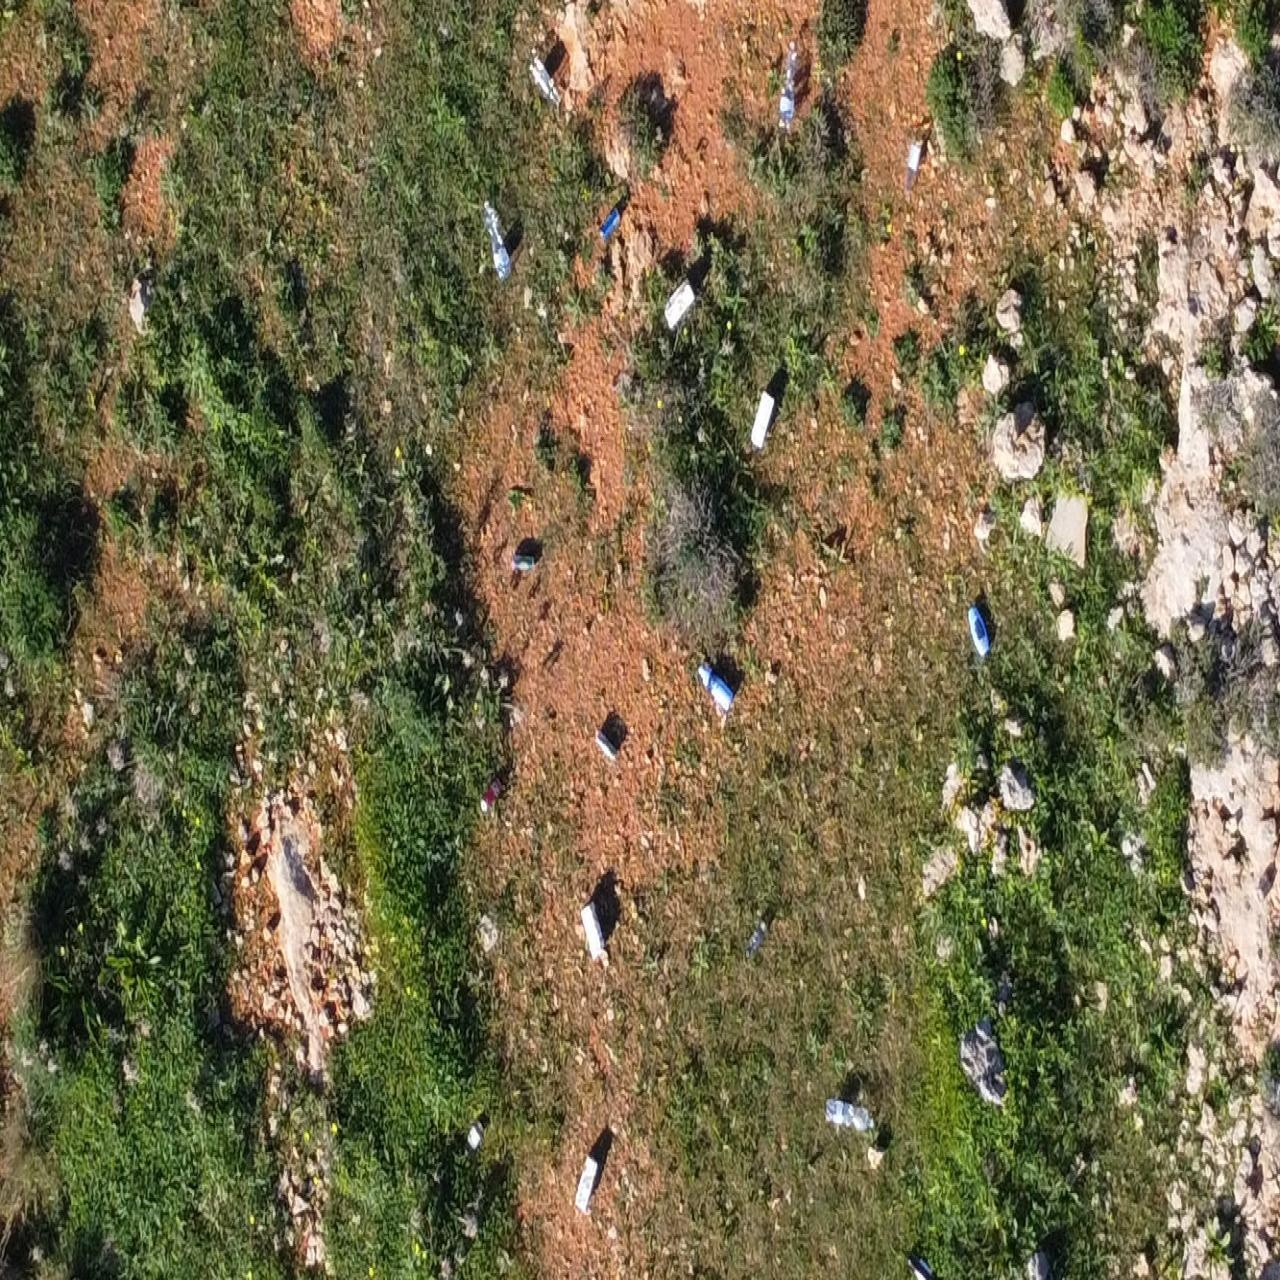
\includegraphics[width=0.48\textwidth, height=5cm]{gray_image.jpg} &
    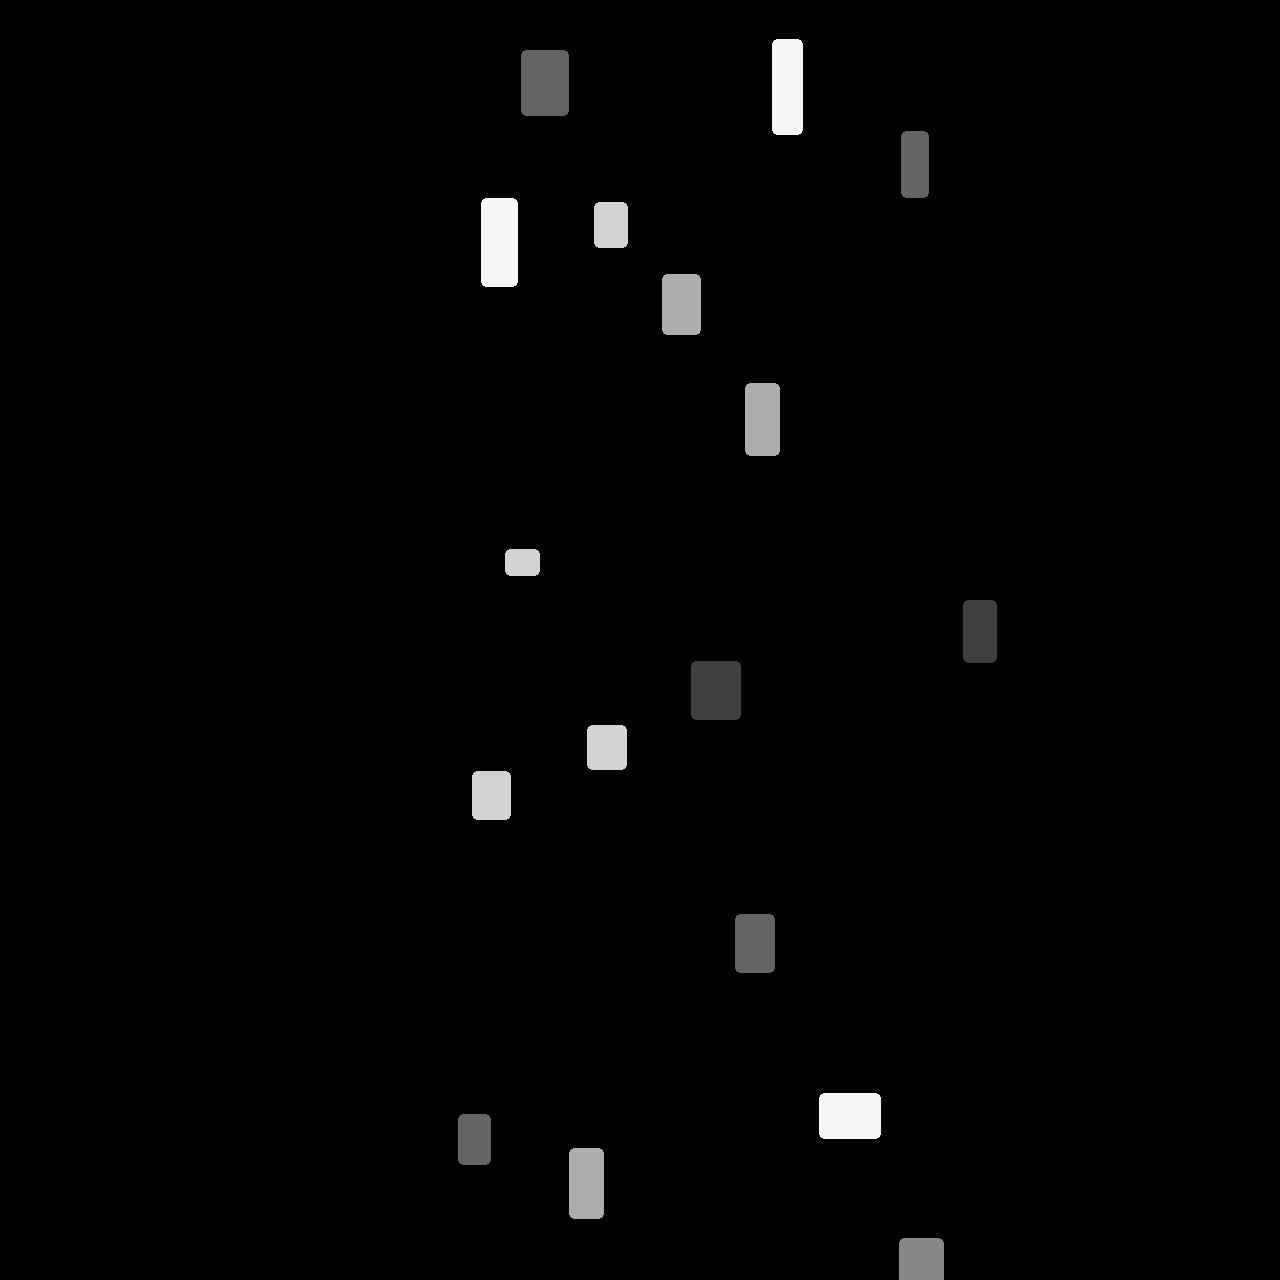
\includegraphics[width=0.48\textwidth, height=5cm]{normal_image.jpg} \\
    \small (a) & \small (b) \\
  \end{tabular}\\
  \caption{Visual illustration of generated privileged information: (a) a three-channel RGB image from the \gls{soda} dataset \cite{soda_dataset}, and (b) the corresponding generated privileged information represented by a single-channel bounding box mask image.}
  \label{fig:privileged_visual}
\end{figure}

The bounding box mask image proposed in this study serves as a structured form of privileged information, developed to support object detection networks across both localisation and classification tasks. The generated image consists of a black background, representing non-object regions. Over this, bounding boxes are drawn to indicate the locations of objects, thereby addressing the localisation problem. To simultaneously encode class-specific information, each bounding box is filled with a distinct shade of grey corresponding to its class label in order to tackle the classification problem. This approach is visually exemplified in Figure \ref{fig:privileged_visual}.
Moreover, a single-channel grayscale format in the range $[0, 255]$ was used to represent the generated privileged information image. This kept the representation simple, preserving essential structure and meaning, without adding extra computational load. This single-channel format was selected in preference to RGB representations, as it simplifies the data without compromising the richness of the information conveyed. The algorithm used to generate this form of privileged input is presented in Algorithm \ref{alg:boundingBoxMask}. Special attention was given to reducing object occlusion within the privileged mask. To achieve this, a sorting step was introduced before rendering the bounding boxes onto the black mask image. The boxes were ordered in descending size, allowing the larger ones to be drawn first. This approach helped to reduce the likelihood of smaller objects being obscured.

% \begin{algorithm}
%     \caption{Generating Bounding Box Mask (Privileged Information) for Object Detection}
%     \label{alg:boundingBoxMask}
%     \begin{algorithmic}
%         \State \textbf{Input:} \( \text{bounding boxes}, \, \text{labels}, \, \text{image width}, \, \text{image height}, \, \text{num classes} \)
%         \State \textbf{Output:} Bounding Box Mask Image (Single Channel)
        
%         \State 1. Create a black image of size \( (\text{image width}, \text{image height}) \) with pixel intensities all 0
%         \State 2. Load the annotations: bounding boxes, labels for multi-label detection
%         \State 3. Create a distinct grayscale colour distribution in the range of 55 to 255 for each label, ensuring no overlapping colours and dark shades
%         \State 4. Sort the annotations by bounding box area (largest first) to prevent object occlusions
        
%         \For{each annotation \( i \) in the set of annotations}
%             \State 5. Extract the bounding box coordinates \( (b_x, b_y, b_w, b_h) \) and label for the current annotation
%             \State 6. Assign a unique grayscale colour to the current label from the predefined colour distribution
%             \State 7. Draw the bounding box on the image using the assigned grayscale colour
%         \EndFor
        
%         \State 8. Save the bounding box mask as a single-channel grayscale image
%     \end{algorithmic}
% \end{algorithm}
\begin{algorithm}
    \caption{Generating Bounding Box Mask (Privileged Information) for Object Detection}
    \label{alg:boundingBoxMask}
    \begin{algorithmic}
        \State \textbf{Input:} Bounding boxes, labels, image width, height, number of classes
        \State \textbf{Output:} Single-channel grayscale bounding box mask
        
        \State 1. Initialise a blank grayscale image of size \( (\text{width}, \text{height}) \)
        \State 2. Load annotations: bounding boxes and class labels
        \State 3. Assign distinct grayscale values in range $[55, 255]$ to each class label to avoid overlap
        \State 4. Sort annotations by bounding box area (descending order) to reduce occlusion
        
        \For{each annotation \( i \)}
            \State 5. Extract bounding box coordinates \( (b_x, b_y, b_w, b_h) \) and label \( l \)
            \State 6. Retrieve grayscale value corresponding to \( l \)
            \State 7. Fill the box region in the image with this value
        \EndFor
        
        \State 8. Save as a single-channel grayscale mask image
    \end{algorithmic}
\end{algorithm}


\section{Deep Learning-Based Object Detection Architectures}
\label{sec:4_distillation_architectures}
% Model Architectures (model selection), explain (don't have to say anything about yolo, used architectures open source, torchvision footnotes, pretrained models trained on COCO just mention) subsection for each one one page for each, 

A structured methodological framework was devised to investigate the influence of \gls{lupi} in object detection and assess whether it provides measurable improvements in accuracy, without necessitating increasingly complex or computationally demanding architectures, to address the first objective (\textbf{O1}). This framework relied on utilising pre-trained models with few structural adjustments, as briefly hinted in the preceding sections, thereby presenting a methodology capable of accommodating the integration of \gls{lupi} into existing detection pipelines to tackle the second objective (\textbf{O2}).
To ensure scientific rigour and relevance, a selection of renowned models was employed to test this hypothesis--models that feature prominently in object detection literature and are also commonly used in litter detection (see Section: \ref{sec:3_litter}). Five architectures were selected for their distinct algorithmic principles and practical relevance: Faster \gls{rcnn} \cite{rcnn}, \gls{ssd} \cite{ssd}, RetinaNet \cite{retinanet}, SSDLite \cite{ssdlite}, and \gls{fcos} \cite{fcos}. All of these models are open-source and publicly available through the \verb|torchvision|\footnote{https://pytorch.org/vision/main/models.html\#object-detection} library, with pre-trained weights sourced from the \gls{coco} dataset. Furthermore, these pre-trained configurations provided a uniform baseline for all subsequent experimental comparisons.

Although the study drew upon the full suite of pre-trained object detection models offered through the \verb|torchvision| \gls{api}, these five were selected particularly for their representational breadth and relevance across differing detection paradigms. Together, these models encapsulate both one-stage and two-stage detection approaches, providing a balanced basis for assessing the contribution of \gls{lupi}. Their selection ensured that any findings are not confined to the characteristics of a single architecture but instead speak to broader trends observable across different model types.

\subsection{Faster Region-based Convolutional Neural Network}
\label{subsec:4_fastercnn}

Faster \gls{rcnn} \cite{fasterrcnn} is an anchor-based detection approach introduced in 2015, and remains a foundational model in two-stage object detection frameworks. It builds upon Fast \gls{rcnn} \cite{fastrcnn} by integrating a \gls{rpn} that shares convolutional features with the detection network, enabling efficient region proposals with minimal computational overhead \cite{fasterrcnn}. By sharing convolutional features between the \gls{rpn} and detection network, this approach enables the model to produce efficient region proposals directly from the feature maps, simplifying the overall detection process \cite{fasterrcnn}.
Subsequent enhancements have incorporated a \gls{fpn} into the architecture, facilitating multi-scale feature representation and improving detection accuracy across varied object sizes. In this study, the implementation utilises the Faster \gls{rcnn} model with a ResNet-FPN backbone, as provided by the \verb|torchvision| library (see Figure \ref{fig:fasterrcnn2}). This configuration combines a ResNet backbone for feature extraction, an \gls{rpn} for generating region proposals, and an \gls{fpn} for handling multi-scale features, all combined through a \gls{roi}-pooling mechanism.

\begin{figure}[!htbp]
    \centering
    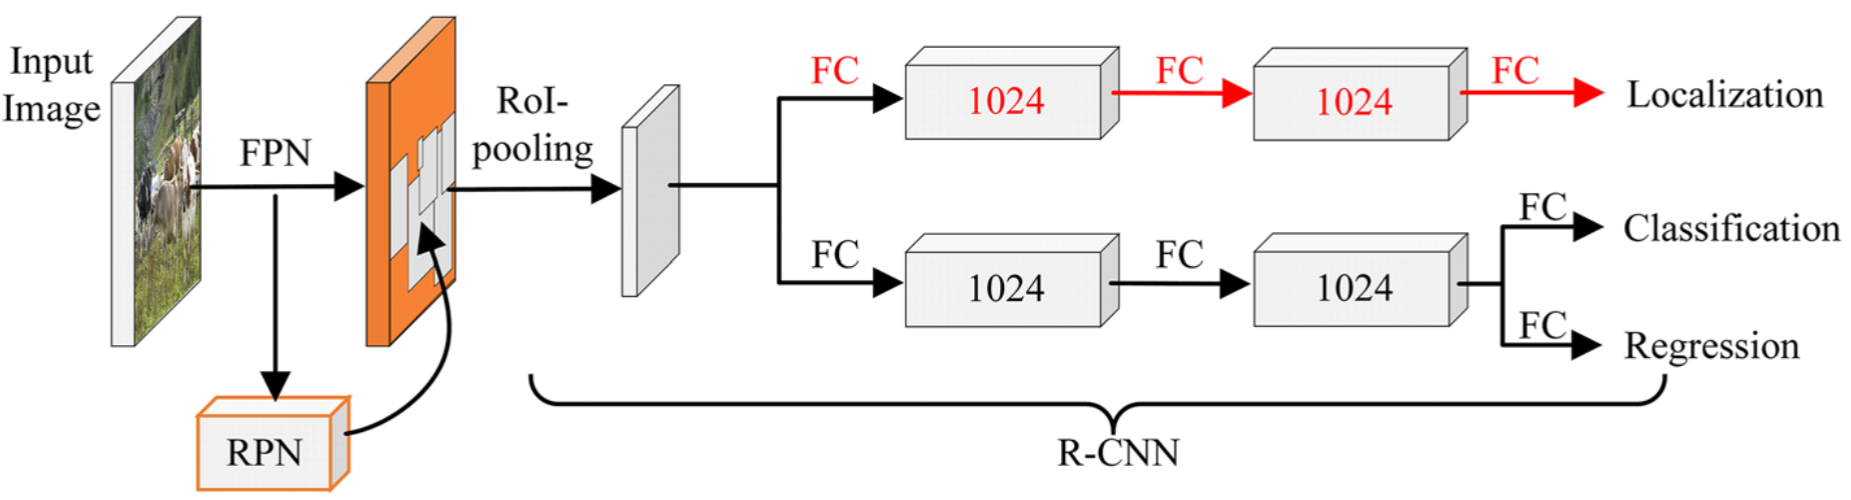
\includegraphics[width=1\columnwidth]{fasterrcnn2.png}
    \caption{Faster \gls{rcnn} architecture with ResNet-50 backbone and \gls{fpn}. The localisation branch, highlighted in red, is separate from the ResNet-FPN structure used in this study, and represents a modification from \cite{fasterrcnn_diagram}. (Source: \cite{fasterrcnn_diagram})}
    \label{fig:fasterrcnn2}
\end{figure}

After the \gls{roi}-pooling stage, the network’s head consists of a single branch that simultaneously handles both classification and bounding box regression. This design reflects the original Faster \gls{rcnn} architecture, where sharing convolutional features between the \gls{rpn} and the detection head enables the model to process both tasks effectively. The branch assigns class labels and refines bounding box coordinates within the same framework, reducing computational overhead and streamlining the detection pipeline \cite{fasterrcnn}.

\subsection{Single Shot MultiBox Detector}
\label{subsec:4_ssd}

Released in 2016, \gls{ssd} \cite{ssd} is a single-stage object detection model that bypasses region proposal networks by directly predicting object classes and box refinements for a fixed set of predefined anchor boxes, known as default boxes. In contrast to two-stage approaches, \gls{ssd} performs all computations in a single pass, which allows for faster inference while maintaining respectable accuracy across varied object scales.
The implementation of \gls{ssd} utilised in this study adopts a modified VGG-16 backbone, discarding the fully connected layers in favour of additional convolutional layers appended after the base network. These added layers progressively reduce spatial resolution, producing multiple feature maps of decreasing size. Each map is responsible for detecting objects at different scales to tackle multi-scale detection.

\begin{figure}[!htbp]
    \centering
    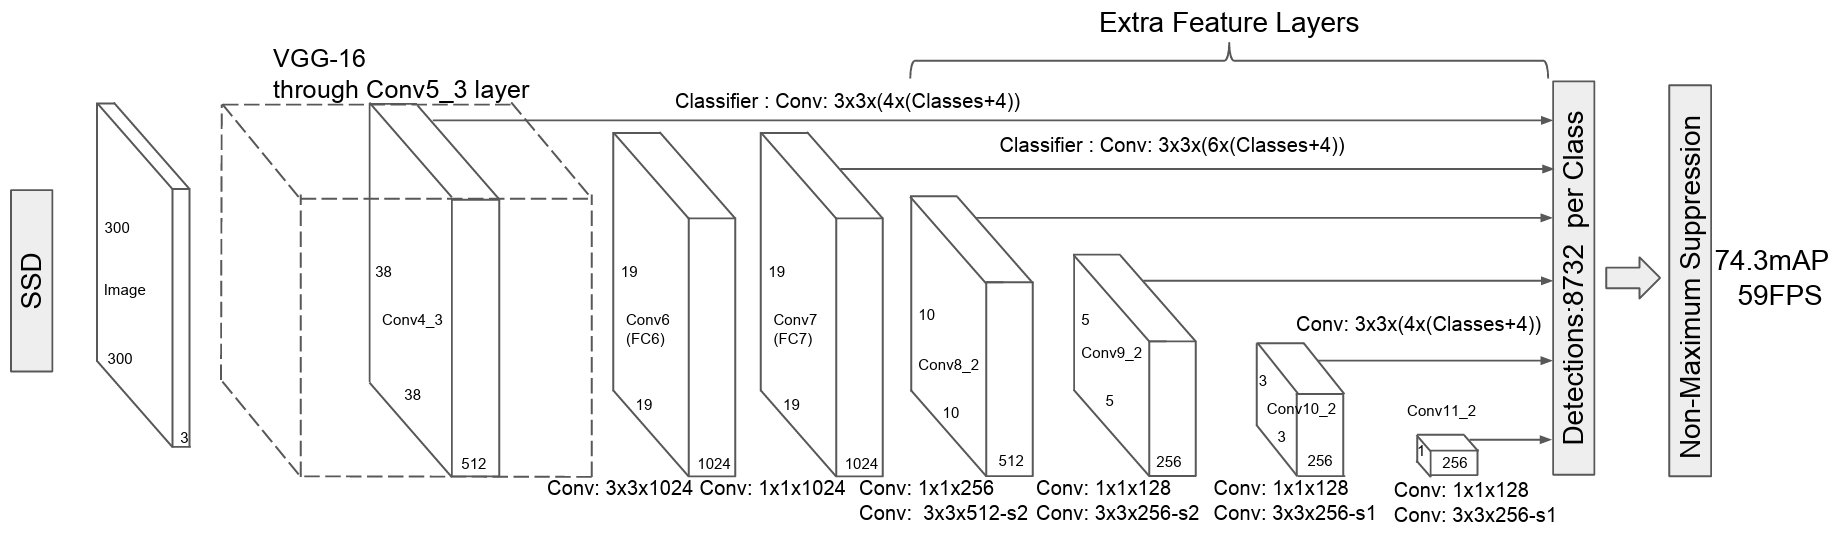
\includegraphics[width=1\columnwidth]{ssd1.png}
    \caption{\gls{ssd} architecture. (Source: \cite{ssd})}
    \label{fig:ssd}
\end{figure}

Default boxes, analogous to anchor boxes, are generated across each feature map based on fixed aspect ratios and scales. The model predicts class probabilities and bounding box offsets using lightweight convolutional heads for each feature map. These heads operate independently across feature levels, allowing for coherent parallel computation. This architectural setup (see Figure \ref{fig:ssd}) allows the model to localise and classify objects in a single forward pass, balancing detection speed with multi-scale representation.

\subsection{RetinaNet}
\label{subsec:4_retinanet}

RetinaNet \cite{retinanet}, introduced in 2017, is a single-stage object detection model designed to address the challenge of foreground–background class imbalance, which often hinders the performance of dense detectors. Unlike two-stage models such as Faster \gls{rcnn}, which generate region proposals before classification, RetinaNet performs both classification and localisation in a single forward pass (see Figure \ref{fig:retinanet}).
The architecture uses a ResNet backbone with a feature pyramid network to capture multi-scale features. Following the \gls{fpn}, it incorporates two parallel subnetworks: one for classifying object categories and another for predicting bounding box coordinates. Notably, a key innovation in RetinaNet is the introduction of focal loss, a variant of cross-entropy loss designed to address foreground–background imbalance by focusing learning on hard, misclassified examples and reducing the influence of easy negatives.

\begin{figure}[!htbp]
    \centering
    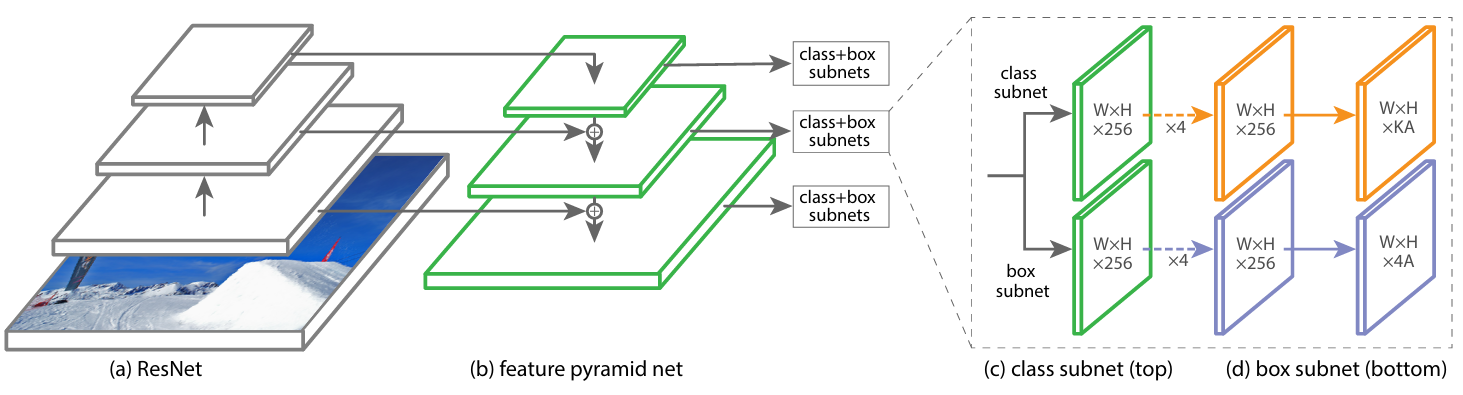
\includegraphics[width=1\columnwidth]{retinanet.png}
    \caption{RetinaNet architecture. (Source: \cite{retinanet})}
    \label{fig:retinanet}
\end{figure}

The model utilises anchor boxes with varying scales and aspect ratios to successfully detect objects of different sizes and shapes. Despite being a single-stage detector, RetinaNet achieves accuracy comparable to more computationally demanding two-stage models, making it a strong baseline in object detection. 
% The RetinaNet network architecture is illustrated in Figure \ref{fig:retinanet}.


\subsection{Single Shot MultiBox Detector Lite}
\label{subsec:4_ssdlite}

Introduced in 2018, SSDLite \cite{ssdlite} represents a streamlined variant of the \gls{ssd}, specifically engineered for deployment on mobile and resource-constrained devices. This model replaces the original \gls{ssd}'s VGG-16 backbone with MobileNetV2, a network characterised by its inverted residual layers and linear bottlenecks, which facilitate efficient feature extraction while maintaining representational capacity \cite{ssdlite}. The integration of MobileNetV2 significantly reduces the computational demands of the model, making it more suitable for real-time applications on devices with limited processing power.

\begin{figure}[!htbp]
    \centering
    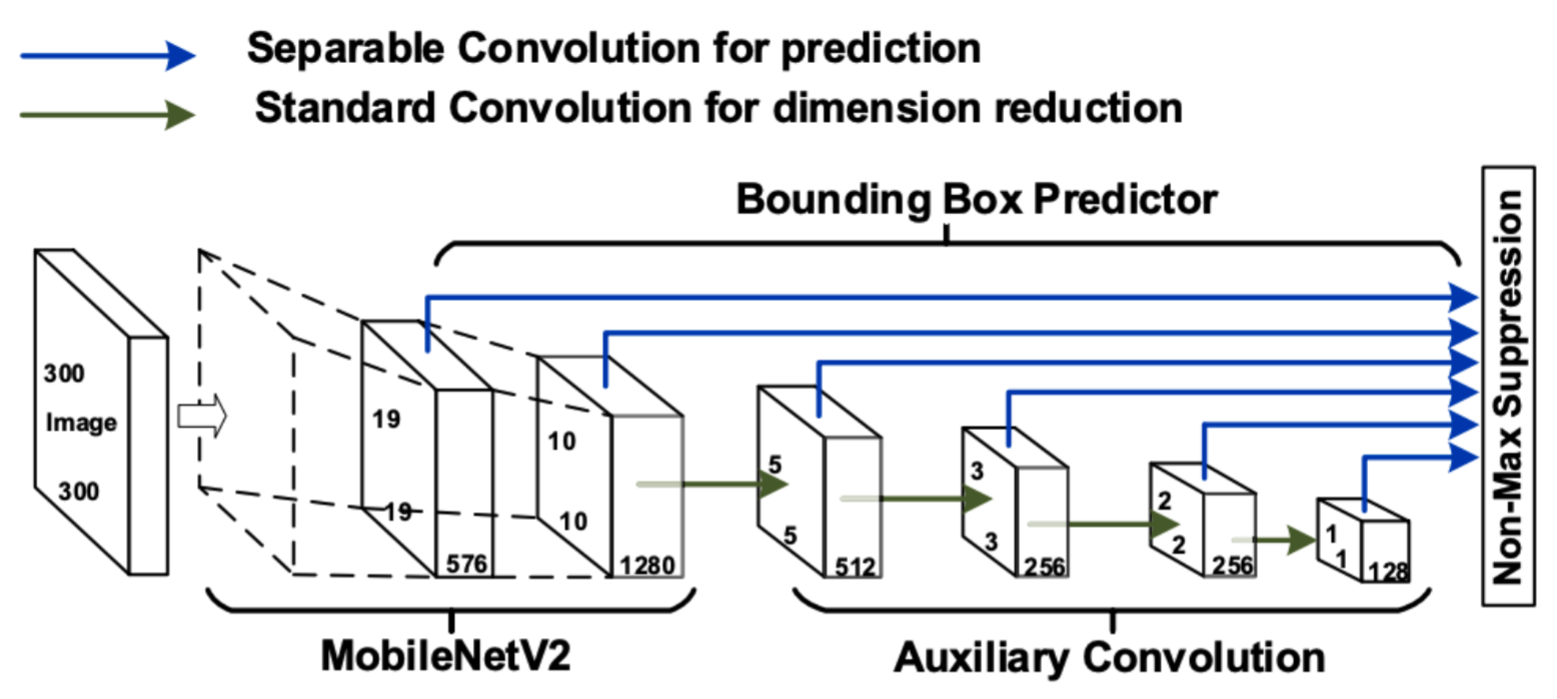
\includegraphics[width=0.8\columnwidth]{ssdlite.png}
    \caption{MobileNetV2-SSDLite architecture. (Source: \cite{ssdlite_diagram})}
    \label{fig:ssdlite}
\end{figure}

A key architectural modification in SSDLite involves the substitution of standard convolutional layers in the detection heads with depthwise separable convolutions (see Figure \ref{fig:ssdlite}). This change aligns with the design principles of MobileNet architectures, where depthwise convolutions are employed to filter input channels independently, followed by pointwise convolutions that combine these outputs \cite{mobilenet}. This approach not only decreases the number of parameters but also accelerates inference time.
Building upon the foundation laid by MobileNetV2 \cite{ssdlite}, subsequent iterations of SSDLite have incorporated MobileNetV3 \cite{mobilenetv3} as the backbone network. MobileNetV3 (see Figure \ref{fig:ssdlite2}) introduces several improvements, including the use of squeeze-and-excitation modules and the h-swish activation function, both of which contribute to improved accuracy and efficiency. These improvements further establish SSDLite as a lightweight detector suitable for deployment in scenarios with limited computational resources, without compromising detection performance \cite{ssdlite}.

\begin{figure}[!htbp]
    \centering
    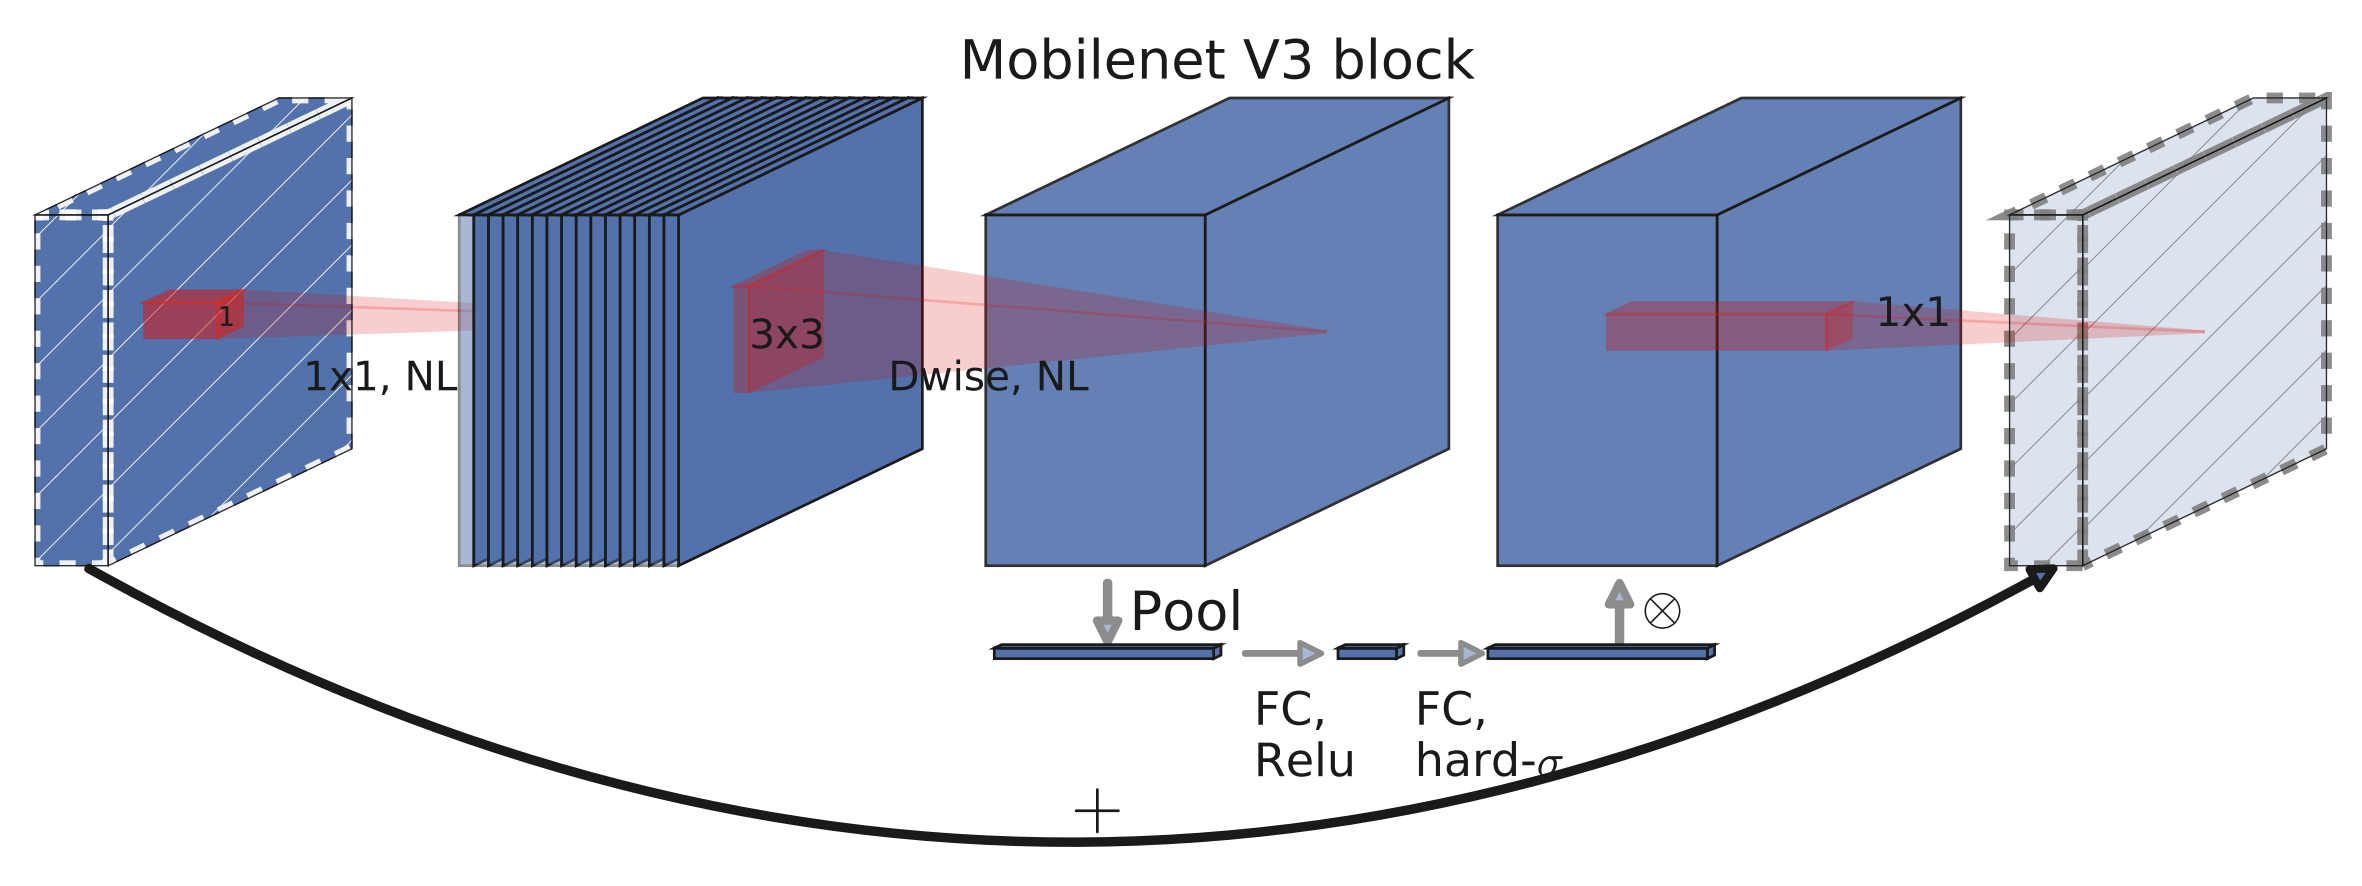
\includegraphics[width=0.9\columnwidth]{mobilenet-v3-block.png}
    \caption{MobileNetV3 architecture. (Source: \cite{mobilenetv3})}
    \label{fig:ssdlite2}
\end{figure}

\subsection{Fully Convolutional One-Stage Object Detection}
\label{subsec:4_fcos}

Introduced in 2019, the \gls{fcos} model \cite{fcos} presents a single-stage detection framework that forgoes the use of anchor boxes, setting it apart from earlier methods reliant on predefined region proposals. Traditional object detectors rely on predefined anchor boxes and require complex computations to evaluate overlaps during training. \gls{fcos} discards this dependency, streamlining the detection process and reducing computational overhead. One of its defining features is the addition of a \textit{centre-ness} branch, which estimates how close a predicted bounding box is to the centre of an actual object. This component contributes an auxiliary loss, enabling the model to focus better on high-quality detections and suppress predictions that lie farther from object centres \cite{fcos}.

\begin{figure}[!htbp]
    \centering
    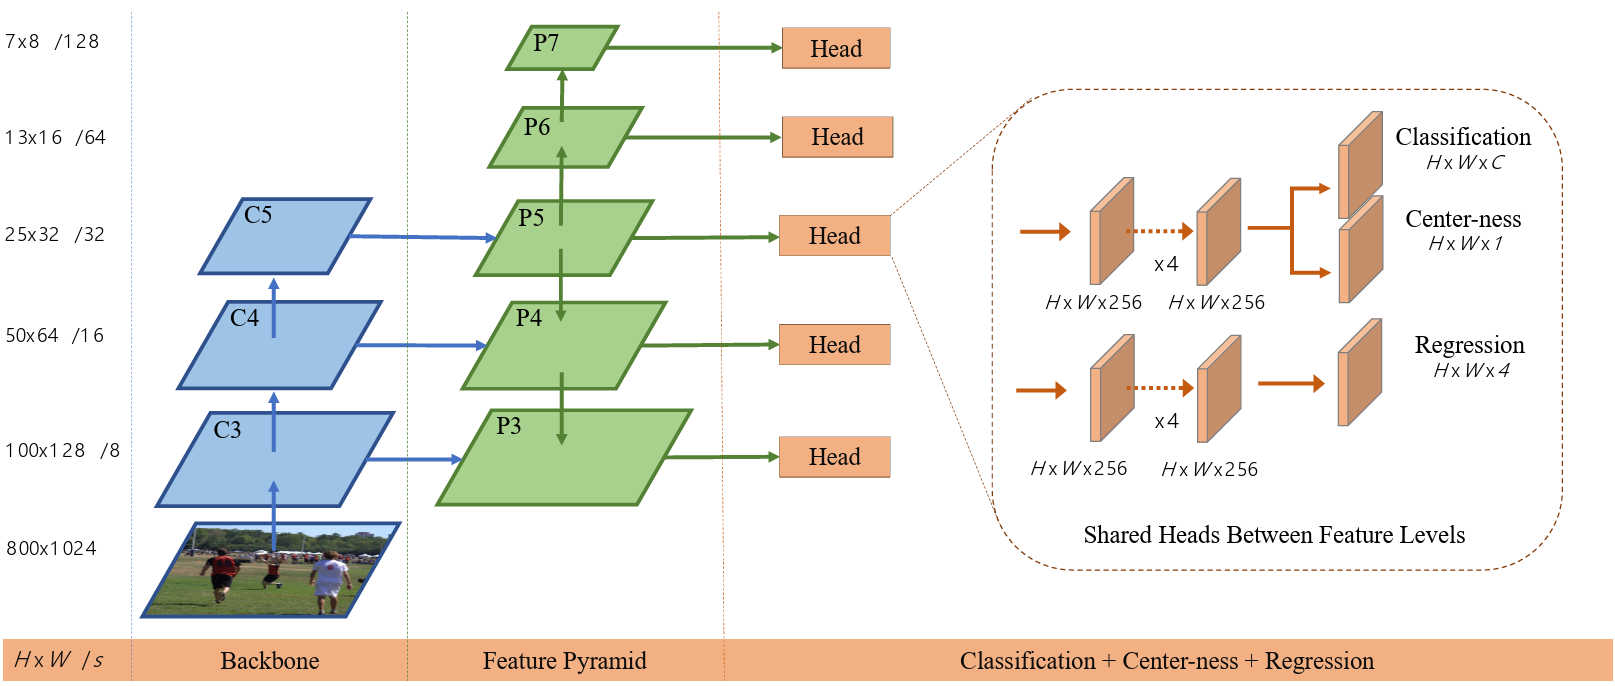
\includegraphics[width=1\columnwidth]{fcos.png}
    \caption{\gls{fcos} architecture. (Source: \cite{fcos})}
    \label{fig:fcos}
\end{figure}

The \gls{fcos} architecture (refer to Figure~\ref{fig:fcos}) is built upon a ResNet-FPN backbone. ResNet serves as the feature extractor, capturing rich spatial and semantic information from input images. The \gls{fpn} complements this by facilitating detection across multiple scales, which is crucial for accurately identifying objects of varying sizes. On top of this backbone, \gls{fcos} incorporates an output head comprising three key elements: a regression branch for predicting bounding box coordinates, a classification branch for object category prediction, and the centre-ness branch mentioned earlier. The classification branch is intentionally split to allow the centre-ness signal to modulate confidence scores, reducing false positives and boosting precision. Collectively, these design choices allow \gls{fcos} to achieve competitive performance without relying on the complex heuristics associated with anchor generation and matching \cite{fcos}. 
% The \gls{fcos} network architecture is illustrated in Figure~\ref{fig:fcos}.

%--

\section{Learning using Privileged Information for Object Detection}
\label{sec:4_lupi4od}

Having defined five key object detection architectures relevant to this study, each based on a distinct detection strategy, and having introduced privileged information as an informative input during training, the next step is to combine these elements. Combining these elements into a single pipeline allows for investigating the \gls{lupi} paradigm within existing object detection frameworks. The approach distinguishes between the privileged information available during training and the limited input used during test time, intending to improve accuracy without increasing model size.

In this setup, privileged information is only available while the model is being trained and not during inference. In light of this, using a teacher–student dynamic becomes necessary, as was done in similar studies \cite{lab2wild, lupi_classification}. The teacher model is trained on both the RGB images (\gls{x}) and the privileged information (\gls{x_star}), along with the target labels (\gls{y}), as is typical in most object detection approaches. With access to this extra information, the teacher can develop a more refined understanding of the target objects.
By contrast, the student model receives only the RGB images (\gls{x}) at inference. During training, it has access to both the images (\gls{x}) and the labels (\gls{y}), but not the privileged information. This mirrors the conditions expected during real-world deployment, so the student must learn without relying on data that will not be present at test time.

The main goal is to improve the student by using the richer knowledge learnt by the teacher. Through distillation, the teacher transfers essential knowledge gained from the privileged information, enabling the student model to achieve a level of performance comparable to that of a model trained with access to additional input--despite the student never having access to that input during inference.
To achieve this, the object detection architectures mentioned earlier can be adapted. By making minor adjustments to the original design, a teacher–student model can be created using the same network architecture. For instance, a RetinaNet teacher model could be used to train a RetinaNet student model.

\subsection{Teacher Network}
\label{subsec:4_teacher}

In this study, a teacher network was implemented to accept both the RGB image and its corresponding bounding box mask as privileged information. This necessitated specific architectural adjustments to a standard object detection model. Conventional models are typically configured to process only three-channel RGB inputs; however, to incorporate the additional single-channel mask, the input layer was modified to accept a four-channel tensor. More generally, the architecture was extended to support inputs with \gls{channels} channels, representing the combined data from the RGB image and any additional privileged sources. As this change directly impacted the initial convolutional layer, its weights required reinitialisation. To maintain consistency with the pre-trained weights and ensure a stable optimisation process, Kaiming Normal initialisation \cite{kaiming} was employed for the modified layer.

\subsection{Student Network}
\label{subsec:4_student}

With the teacher network established, the subsequent step involved defining the student network. While the student learns under the supervision of the teacher, it does not receive any privileged information as input. Consequently, the input layer of the student network remained unaltered, allowing the direct use of a standard pre-trained object detection model. To incorporate teacher supervision during training, however, the student’s loss function had to be adjusted to include a distillation term, as described in Equation \ref{eq:lupi_loss_function}. To enable meaningful feature-level distillation, this approach required the selection of a shared internal layer from both networks, one that captures semantically rich representations and allows for direct comparison. In this study, the final backbone layer was selected for distillation, in line with existing approaches in this area \cite{lab2wild, lupi_distillation, distillation2}. Specifically, for architectures such as Faster \gls{rcnn}, RetinaNet, and \gls{fcos}, which rely on the ResNet-FPN backbone, this corresponded to the final convolutional layer preceding the \gls{fpn}. The feature layer used for distillation in \gls{ssd}, and SSDLite was taken just before the auxiliary detection heads, corresponding to the final layer of the VGG-16 and MobileNetv3 backbones, respectively.

Once the appropriate layer was selected, the corresponding latent feature representations were extracted during training from both the student and the teacher. These outputs were then flattened into vectors, allowing for a similarity comparison using the Cosine Distance (\gls{D}) function. This metric quantifies the angular divergence between the two feature vectors, offering a precise scalar measure of their alignment in feature space. The resulting distance value was then integrated into the student’s total loss function. As outlined in Equation \ref{eq:lupi_loss_function}, an \gls{alpha} parameter controls the influence of this distillation loss, balancing the learning from direct supervision against the soft guidance offered by the teacher.

\subsection{Proposed Architecture}
\label{subsec:4_architecture}
% Grazzi Sinjur Alla, Ahfirli Sinjur Alla, u Ismaghni Sinjur Alla

Bringing together all the elements described, the incorporation of privileged information into any object detection model can be formally represented through the architecture depicted in Figure \ref{fig:lupi_architecture}. This method rests on two core alterations: adapting the teacher network to process both RGB images and the corresponding privileged input and introducing a loss adjustment in the student model to enable distillation. These adjustments are deliberately kept minimal to prevent unnecessary architectural complexity or increased computational demands. The required changes are confined to modifying the input layer of the teacher model and integrating a distillation mechanism during the student training. Moreover, generating the privileged information, such as bounding box masks, remains a simple and direct process.
% \begin{figure}[!htbp] % Overflow since problem with small font
%     \centering
%     \hspace*{-0.1\textwidth}  % Adjust the negative value as needed to slightly overflow
%     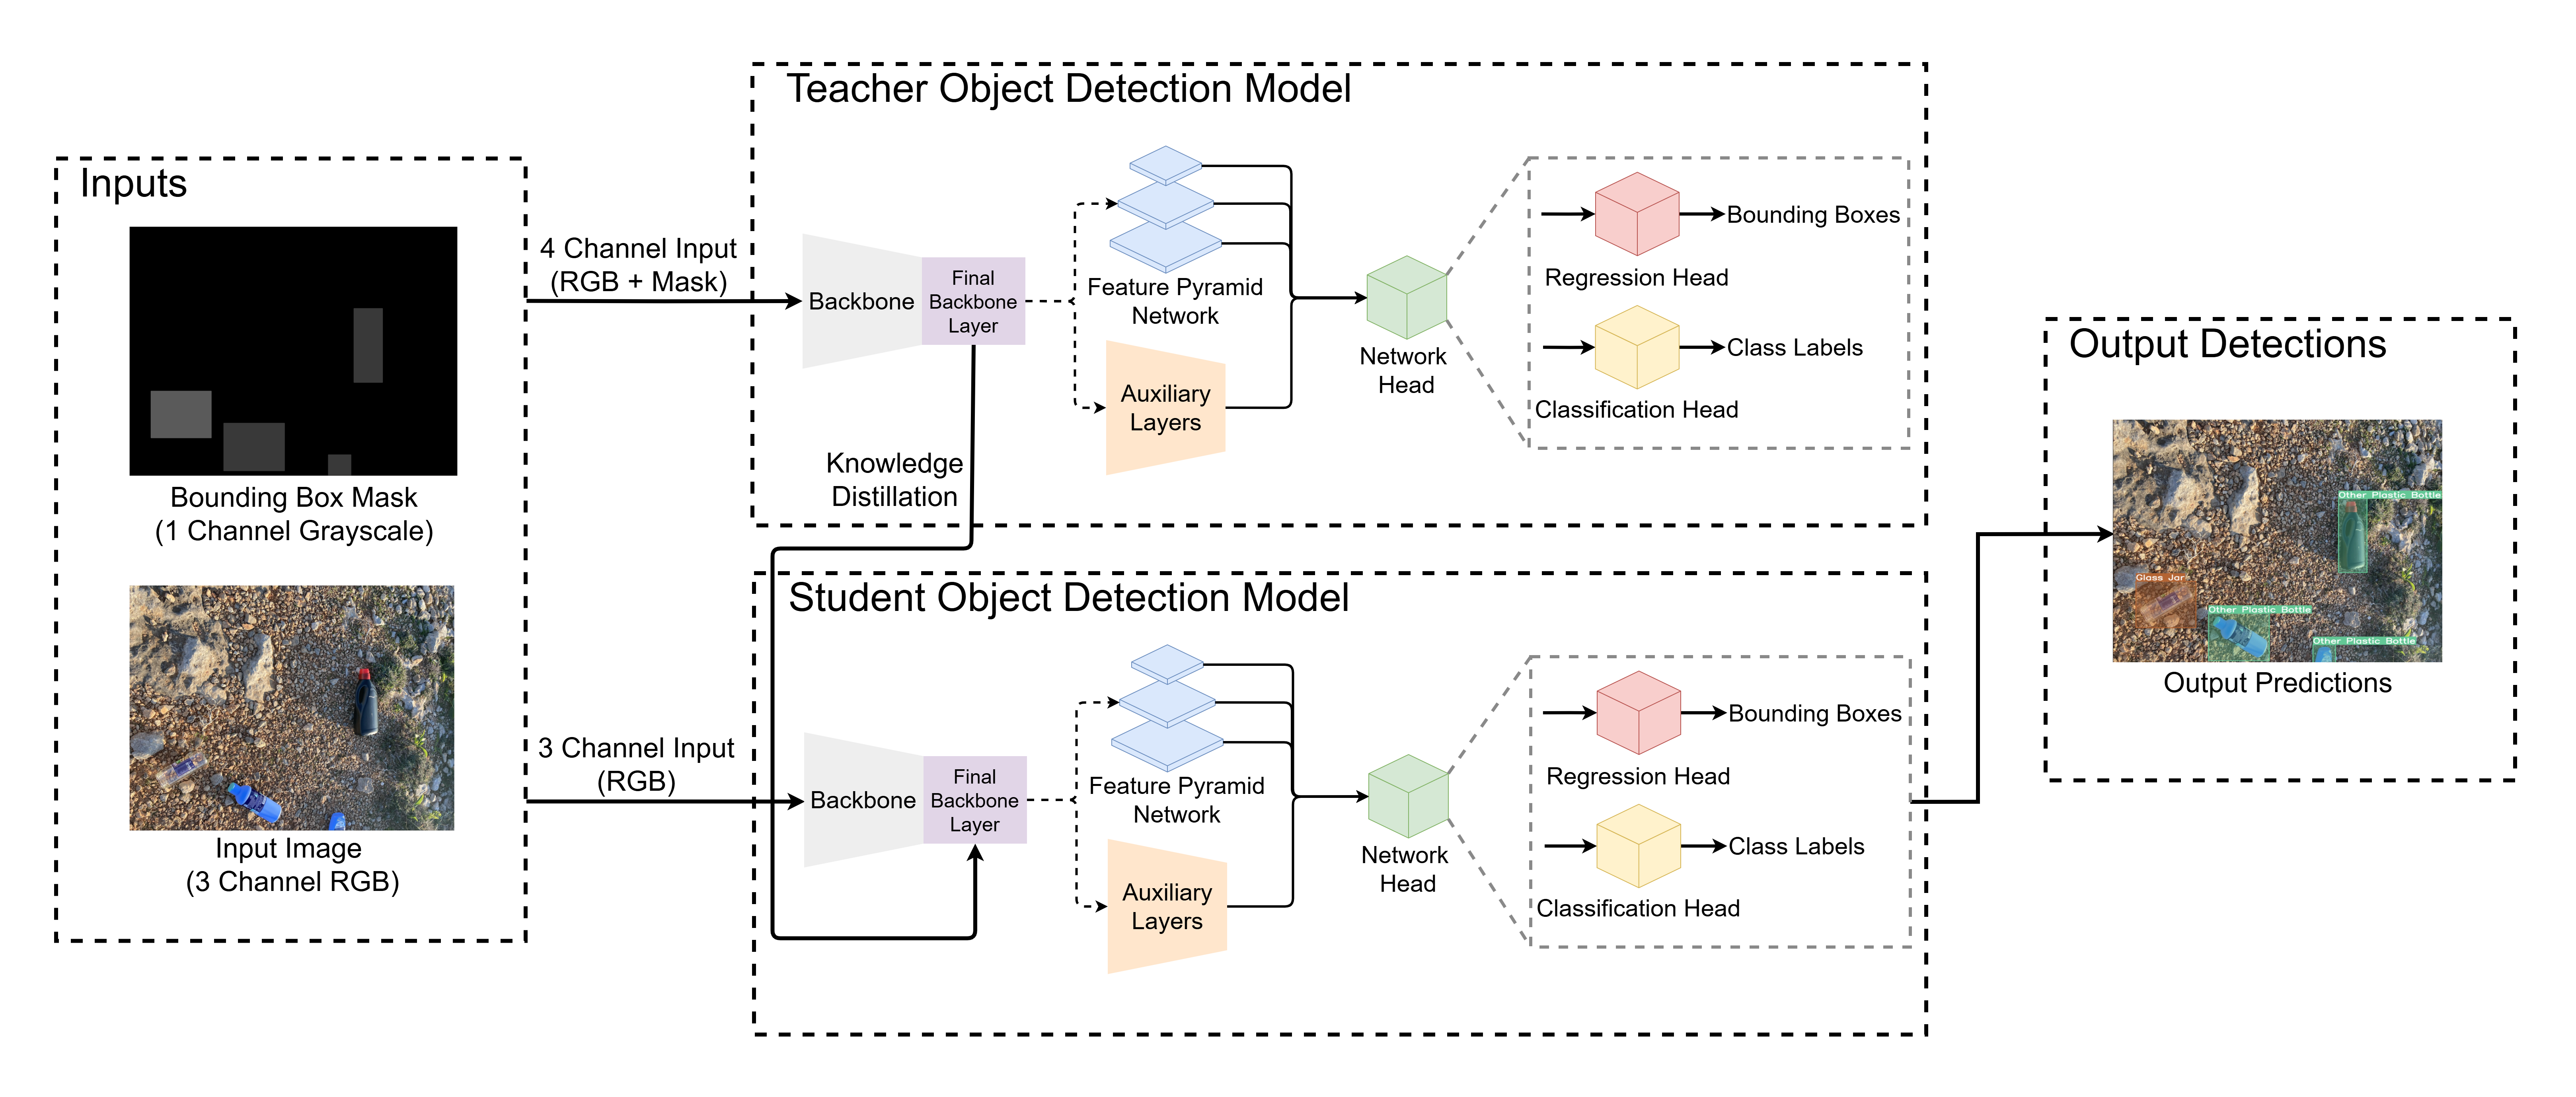
\includegraphics[width=1.2\textwidth]{Architecture LUPIv2.png}
%     \caption{Architecture of the object detection models, illustrating the use of the LUPI paradigm with RGB and bounding box mask inputs, the teacher and student networks, the final backbone layer for knowledge distillation, and the output predictions.}
%     \label{fig:lupi_architecture}
% \end{figure}
\begin{figure}[ht]
    \centering
    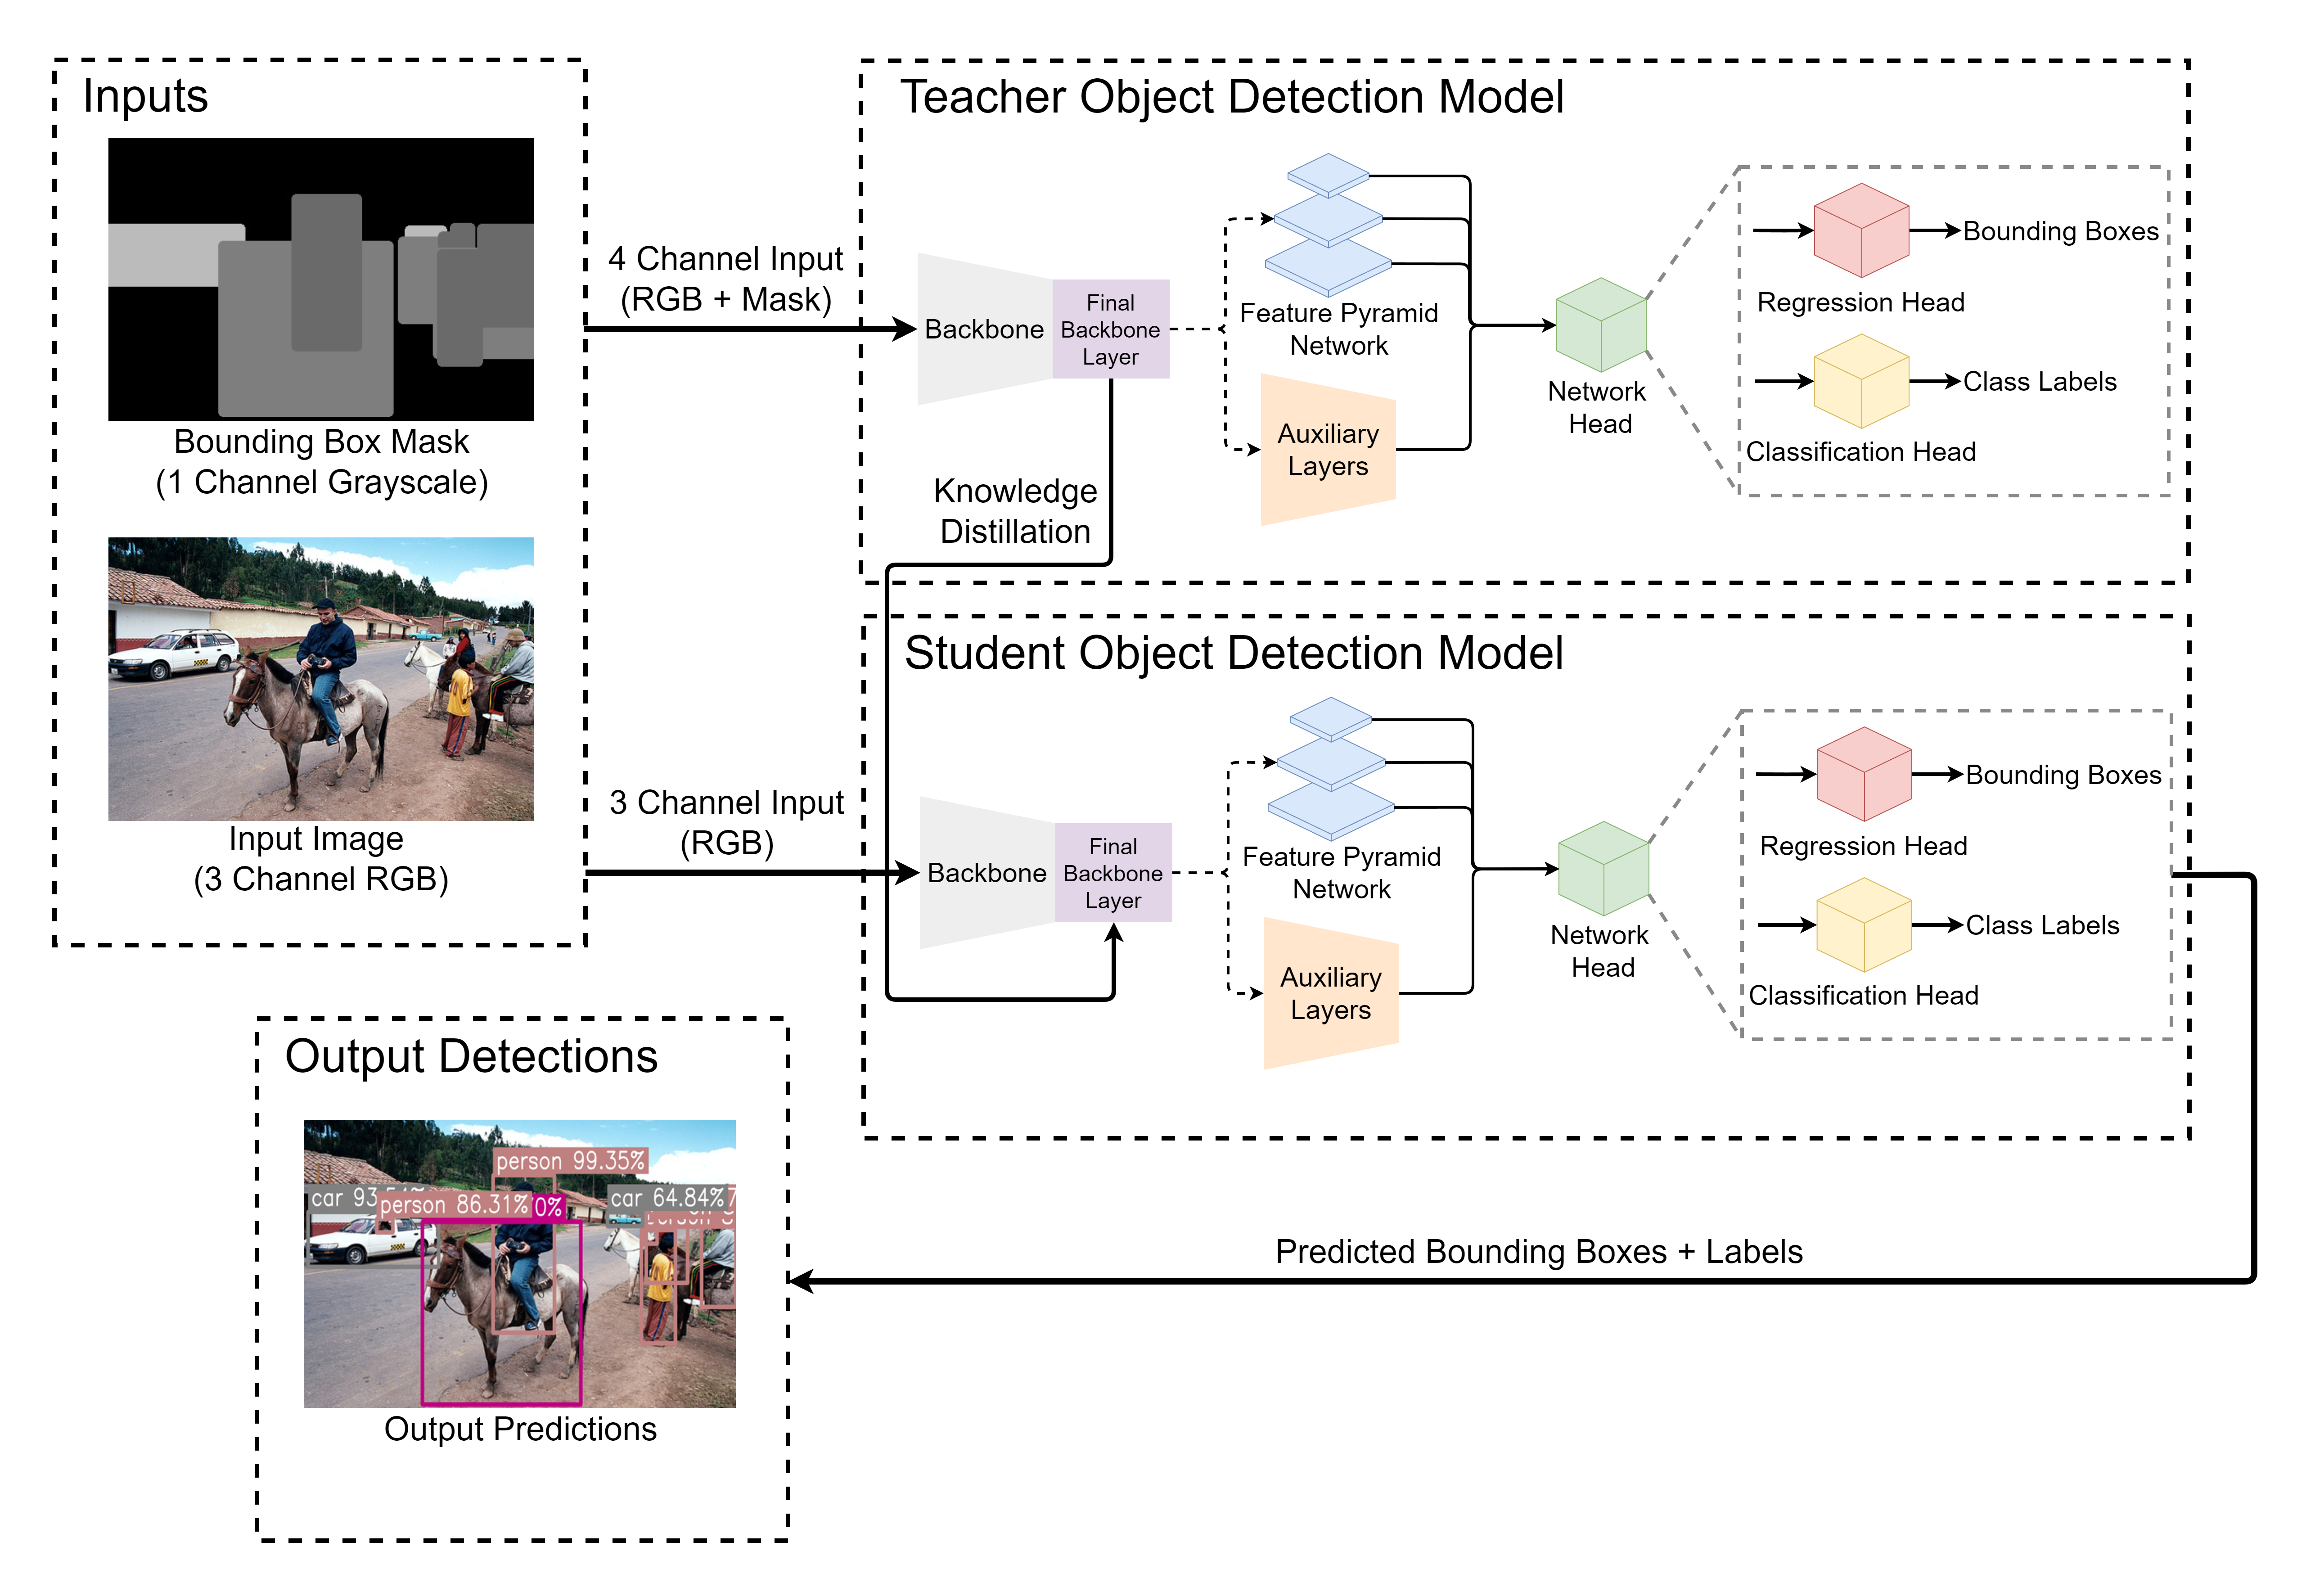
\includegraphics[width=1\textwidth]{Architecture LUPIv3.png}
    \caption{General architecture for integrating the \gls{lupi} paradigm into any object detection model. The diagram illustrates the incorporation of both RGB images and bounding box masks as inputs to the teacher network, the use of a standard RGB input for the student network, the selection of the final backbone layer for knowledge distillation, and the generation of output predictions from the student model.}
    \label{fig:lupi_architecture}% Resized to 200%
\end{figure}

Training an optimised detection model in this study began with the teacher network, which was configured to learn from a richer four-channel input composed of RGB data and privileged information. Once the teacher was trained, its parameters were frozen, and it served as a guide for the student model. During this training phase, the student processed only the standard RGB images, ensuring no modifications to the existing detection architecture. Feature representations were drawn from the final layer of the backbone in both networks. Using identical architectures for the teacher and student simplifies implementation, as it guarantees that the resulting feature vectors are dimensionally aligned and directly comparable.

The similarity between these latent feature representations was measured using a cosine distance function (see Equation \ref{eq:cosine_distance}), producing a distillation loss that captures the degree of alignment between the student and teacher. The distillation loss was first computed and then backpropagated through the student model, alongside the standard detection losses. A tunable parameter, \gls{alpha}, controls how much the teacher’s guidance influences the total loss during training. Upon completing this training phase, the teacher model is no longer needed. However, despite being trained without access to privileged information at inference time, the resulting student model benefits from the guided supervision afforded during training.

\section{Training Parameters}
\label{sec:4_training_params}
% Glorja lil Missier, lil Iben u lil-Ispirtu s-Santu. Kif kien mill-bidu issa u dejjem, ghal dejjem ta' dejjem. Amen

To evaluate the proposed methodology across the five selected object detection models, a uniform experimental training protocol was employed throughout, in alignment with the second objective (\textbf{O2}). The primary aim was to determine whether the integration of the \gls{lupi} framework could yield improvements in detection accuracy without imposing additional computational demands on the baseline architectures. To ensure that any observed improvements in performance could be attributed solely to the inclusion of \gls{lupi}, the training configuration was intentionally kept simple and consistent. Each model was trained for $100$ epochs using the \gls{adam} optimiser \cite{adam_optimizer}, with a fixed learning rate of \(1 \times 10^{-3}\).
Preliminary tests compared alternative optimisers and learning rates \cite{sgd_optimizer}. Although the \gls{sgd} optimiser was initially considered, \gls{adam} achieved comparable convergence to the same minimum but with greater efficiency. Various learning rates were also explored, including $0.1, 0.01, 0.001,$ \(1 \times 10^{-3}\), and \(1 \times 10^{-4}\). Among these, \(1 \times 10^{-3}\) consistently provided the most stable convergence across the selected models. 
In addition, an early stopping callback was applied based on validation loss, with a patience threshold of eight epochs. A model checkpointing mechanism was also used to retain the weights corresponding to the best-performing epoch, thereby minimising the risk of overfitting.
Moreover, following standard practice when training object detection models for a given application or dataset \cite{yolov12, soda_dataset, fasterrcnn, yolov10}, all models were initialised with pre-trained weights from the \gls{coco} dataset. The detection heads were subsequently adapted to match the number of target categories present in the specific dataset used during training.

\section{Pre-processing Steps}
\label{sec:4_preprocessing}
% Sliema ghalik Marija, bil-Grazzja mimlija, Imbierek il frott tal guf tieghek Gesu', Qaddisa Marija Omm Alla, Itlob ghalina l-mindibin, issa u fis siegha tal-mewt taghna. Amen

In addition to the training parameters, a consistent set of preprocessing steps was applied across all experiments to maintain comparability of results. These transformations applied to the input images of the detection networks include image normalisation, resizing, and per-channel standardisation, each of which is outlined in detail below.

\subsection{Min-Max Normalisation}
\label{subsec:4_normalisation}

The initial step involves normalising the image pixels to a uniform scale. This is done to ensure equal weighting across all image inputs and channels. Both the RGB inputs and the additional privileged information channels are scaled using Min-Max normalisation \cite{min_max_normalisation}, as described below:

\begin{equation} \label{eq:min_max}
I_{\text{norm}} = \frac{I - I_{\text{min}}}{I_{\text{max}} - I_{\text{min}}} .
\end{equation}

\noindent Here, \gls{image} refers to the original image, \gls{imin} and \gls{imax} are the minimum and maximum pixel intensity values computed across the entire dataset for each respective channel. The inputs are scaled to lie within the range $[0, 1]$, thereby normalising the input space for both the teacher and student networks. Crucially, normalisation is performed separately for the RGB images and the privileged information channels to maintain the distinct statistical properties of each modality. 

\subsection{Image Resizing}
\label{subsec:4_resizing}

Following normalisation, all images are resized to a fixed resolution of $800 \times 800$ pixels. This resizing step allows for the formation of input tensors with consistent dimensions, a prerequisite for batch training in convolutional neural networks. The resolution of $800$ pixels was selected as a compromise across the models employed in this study.
Although models such as \gls{ssd} and SSDLite typically operate on smaller input resolutions (e.g., $300 \times 300$ or $320 \times 320$), detectors like Faster \gls{rcnn}, RetinaNet, and \gls{fcos} adopt a minimum resize of $800$ pixels. The choice of a larger image resolution also contributes to preserving fine-grained features, which is especially relevant for detecting small-scale objects that might otherwise lose distinctive characteristics if downsampled excessively.

\subsection{Channel-Wise Standardisation}
\label{subsec:4_standardisation}

The final step in the pre-processing pipeline involves statistical normalisation by subtracting the channel-wise mean and dividing by the standard deviation. These parameters are computed over the training dataset and are applied individually to each channel, including both RGB and privileged input. This transformation ensures zero-mean and unit-variance inputs, which helps stabilise training and accelerate convergence \cite{min_max_normalisation}. This standardisation is carried out automatically by the model during training, based on mean and standard deviation values calculated from the specified dataset. The computed mean and standard deviation values for each training dataset and input channel are summarised in Table~\ref{tab:channel_stats}, with the corresponding datasets explored in Section~\ref{sec:4_datasets}.

\begin{table}[ht]
    \centering
    \begin{tabular}{llcc}
        \toprule
        \textbf{Dataset} & \textbf{Channel} & \textbf{Mean} & \textbf{Standard Deviation} \\
        \midrule
        \multirow{4}{*}{\textbf{SODA Litter (01m Altitude)}} 
            & Red               & 0.434 & 0.261 \\
            & Green             & 0.406 & 0.249 \\
            & Blue              & 0.320 & 0.238 \\
            & Bounding Box Mask & 0.144 & 0.135 \\
        \midrule
        \multirow{4}{*}{\textbf{SODA Litter (All Altitudes)}} 
            & Red               & 0.467 & 0.255 \\
            & Green             & 0.430 & 0.240 \\
            & Blue              & 0.357 & 0.233 \\
            & Bounding Box Mask & 0.021 & 0.129 \\
        \midrule
        \multirow{4}{*}{\textbf{Pascal VOC 2012}} 
            & Red               & 0.452 & 0.275 \\
            & Green             & 0.431 & 0.273 \\
            & Blue              & 0.399 & 0.284 \\
            & Bounding Box Mask & 0.142 & 0.216 \\
        \bottomrule
    \end{tabular}
    \caption{Channel-wise mean and standard deviation values for the Red, Green, Blue, and Bounding Box Mask channels, computed over the training sets of the Pascal VOC 2012 and SODA Litter datasets.}
    \label{tab:channel_stats}
\end{table}

Overall, these pre-processing transformations were kept deliberately minimal, consistent, and aligned with the general standards in object detection research to ensure that the influence of the \gls{lupi} methodology could be fairly and transparently evaluated without extraneous confounding factors.

\section{Post-processing Steps}
\label{sec:4_postprocessing}
% Missierna li into fis Smewwiet, Jitqaddes Ismek, tigi Saltnatek, Ikun dak li tried into, hekk fis Semma Hekk da fl-art. Hobzna ta' kuljum ghatina illum, Ahfrilna dnubietna Bhalma Nahfru dak li Huwa Hati' Ghalina. La ddahalniex fit tigrib izda ehlisna mid deni. Amen

In addition to the pre-processing techniques applied to the input images, a consistent post-processing step was introduced to ensure uniformity across all five selected models. This step employed non-maximum suppression \cite{nms}, a widely used method for refining object detection results by eliminating redundant predictions.
The suppression process ranks all predicted bounding boxes according to their confidence scores. When two or more boxes significantly overlap, only the one with the highest score is retained. In this study, the significant overlap was defined using an \gls{iou} threshold of $0.5$. Any box exceeding this level of overlap with a higher-scoring prediction was removed by the \gls{nms}.
Applying this method consistently was essential for a fair evaluation. Some of the chosen models already had \gls{nms} integrated internally, while others required an external implementation. By enforcing a common post-processing step, the outputs became directly comparable, regardless of any differences in model architecture.

\section{Datasets}
\label{sec:4_datasets}
% definition of dataset - check old thesis
% litter detection for uav hard problem, 
% uav based dataset highlighted in lit review chosen, but HAIDA annotations could not be downloaded
% mention why they were selected available etc. . ., mention roboflow
% images for each one

The object detection problem, which is regarded as a supervised learning task, necessitates the use of datasets for both training and validating detection models. These datasets typically consist of image sequences annotated with ground truth bounding boxes and class labels, specifying the type and location of each object \cite{pascal-voc-2012, coco}.
To evaluate the proposed methodological architecture in alignment with the third objective (\textbf{O3}), \gls{uav}-based litter detection was chosen as the target problem to assess the feasibility of the proposed approach. This problem presents a considerable challenge due to the need to detect small objects in varied terrain and under differing altitudes \cite{soda_dataset}. Moreover, the complexity of this task makes it a suitable benchmark for evaluating both the generalisability and precision of the proposed framework.

Currently, only four \gls{uav}-based litter detection datasets are available (see Table \ref{tab:lit_review}): \gls{bdw} \cite{bdwdataset}, UAVVaste \cite{uavvaste}, HAIDA \cite{haida}, and \gls{soda} \cite{soda_dataset}. Among these datasets, \gls{bdw}\footnote{https://universe.roboflow.com/bottles-in-the-wild}, UAVVaste\footnote{https://universe.roboflow.com/mcast/uavvaste-avcle}, and \gls{soda}\footnote{https://universe.roboflow.com/soda-dataset/} are accessible through the Roboflow dataset annotation platform. Although the HAIDA dataset is publicly available on Github\footnote{https://github.com/LiaoSteve/HAIDA-Trash-Dataset-High-Resolution-Aerial-image}, it could not be used due to inaccessible annotations. As a result, the evaluation focused on the three datasets available through Roboflow. In addition, the well-established Pascal VOC 2012 dataset \cite{pascal-voc-2012}, also accessible on Roboflow\footnote{https://public.roboflow.com/object-detection/pascal-voc-2012/1}, was included to give a broader perspective. It was chosen to test the proposed approach for multi-label detection across a larger variety of classes.


\subsection{SODA: Small Objects at Different Altitudes}
\label{subsec:4_soda}

As discussed in Subsection \ref{subsec:3_sodadataset}, \gls{soda} serves as a representative \gls{uav}-based litter detection dataset. It includes six litter classes and contains image subsets captured at a range of altitudes, which reflects more realistic operating conditions for \gls{uav}-based detection.
However, as shown in Table \ref{tab:soda_annotation_summary}, one of the key issues with this dataset is class imbalance. Certain categories, such as \textit{Drink Can} and \textit{Clear Plastic Bottle}, contain significantly more annotations than others. There is also an uneven distribution of images across altitudes, with noticeably fewer samples at higher elevations.
Despite these limitations, \gls{soda} remains a valuable dataset in this area of research. Among the three datasets selected in this study, \gls{soda} covers the widest range of altitudes.

\begin{table}[ht]
    \centering
    \begin{adjustbox}{max width=\textwidth}
    \renewcommand{\arraystretch}{2}%1.5
    \begin{tabular}{|c|c|c|c|c|c|c|c|c|}
        \hline
        \textbf{\gls{agl} (m)} & \textbf{Total Images} & \textbf{Total Annotations} & \textbf{Drink Can} & \textbf{Clear Plastic Bottle} & \textbf{Glass Bottle} & \textbf{Other Plastic Bottle} & \textbf{Drink Carton} & \textbf{Glass Jar} \\
        \hline \hline
        1  & 452 & 712  & 256 & 180 & 96  & 71  & 54  & 55 \\
        \hline
        5  & 202 & 1839 & 837 & 429 & 183 & 152 & 136 & 102 \\
        \hline
        10 & 50  & 1138 & 491 & 268 & 128 & 106 & 88  & 57 \\
        \hline
        15 & 35  & 956  & 434 & 232 & 93  & 87  & 67  & 43 \\
        \hline
        20 & 30  & 763  & 324 & 199 & 68  & 79  & 57  & 36 \\
        \hline
        25 & 30  & 709  & 327 & 174 & 46  & 79  & 57  & 26 \\
        \hline
        30 & 30  & 602  & 270 & 149 & 36  & 82  & 55  & 10 \\
        \hline \hline
        \textbf{Total (Incl. 1m)} & \textbf{829} & \textbf{6719} & \textbf{2939} & \textbf{1631} & \textbf{650} & \textbf{656} & \textbf{514} & \textbf{329} \\
        \hline
        \textbf{Total (Excl. 1m)} & \textbf{377} & \textbf{6007} & \textbf{2683} & \textbf{1451} & \textbf{554} & \textbf{585} & \textbf{460} & \textbf{274} \\
        \hline
    \end{tabular}
    \renewcommand{\arraystretch}{1}%1.5
    \end{adjustbox}
    \caption{Summary of annotated objects across different altitudes \gls{agl} in the \gls{soda} dataset. (Source: \cite{soda_dataset})}
    \label{tab:soda_annotation_summary}
\end{table}

In the original publications that introduced the SODA dataset and used it for training detection models \cite{soda_dataset, detect_litter}, the authors adopted a tiling technique \cite{tiling, sahi_detection}. This method aimed to improve the detection of small objects, particularly in images taken at higher altitudes, by magnifying specific regions. In \cite{detect_litter}, they applied a 5$\times$5 tiling strategy, resizing each tile to 640$\times$640 pixels to match the input dimensions required by the \gls{yolo}v8 \cite{yolov8} network employed in their study.

\begin{figure}[!htbp]
  \centering

  % Full-width image
  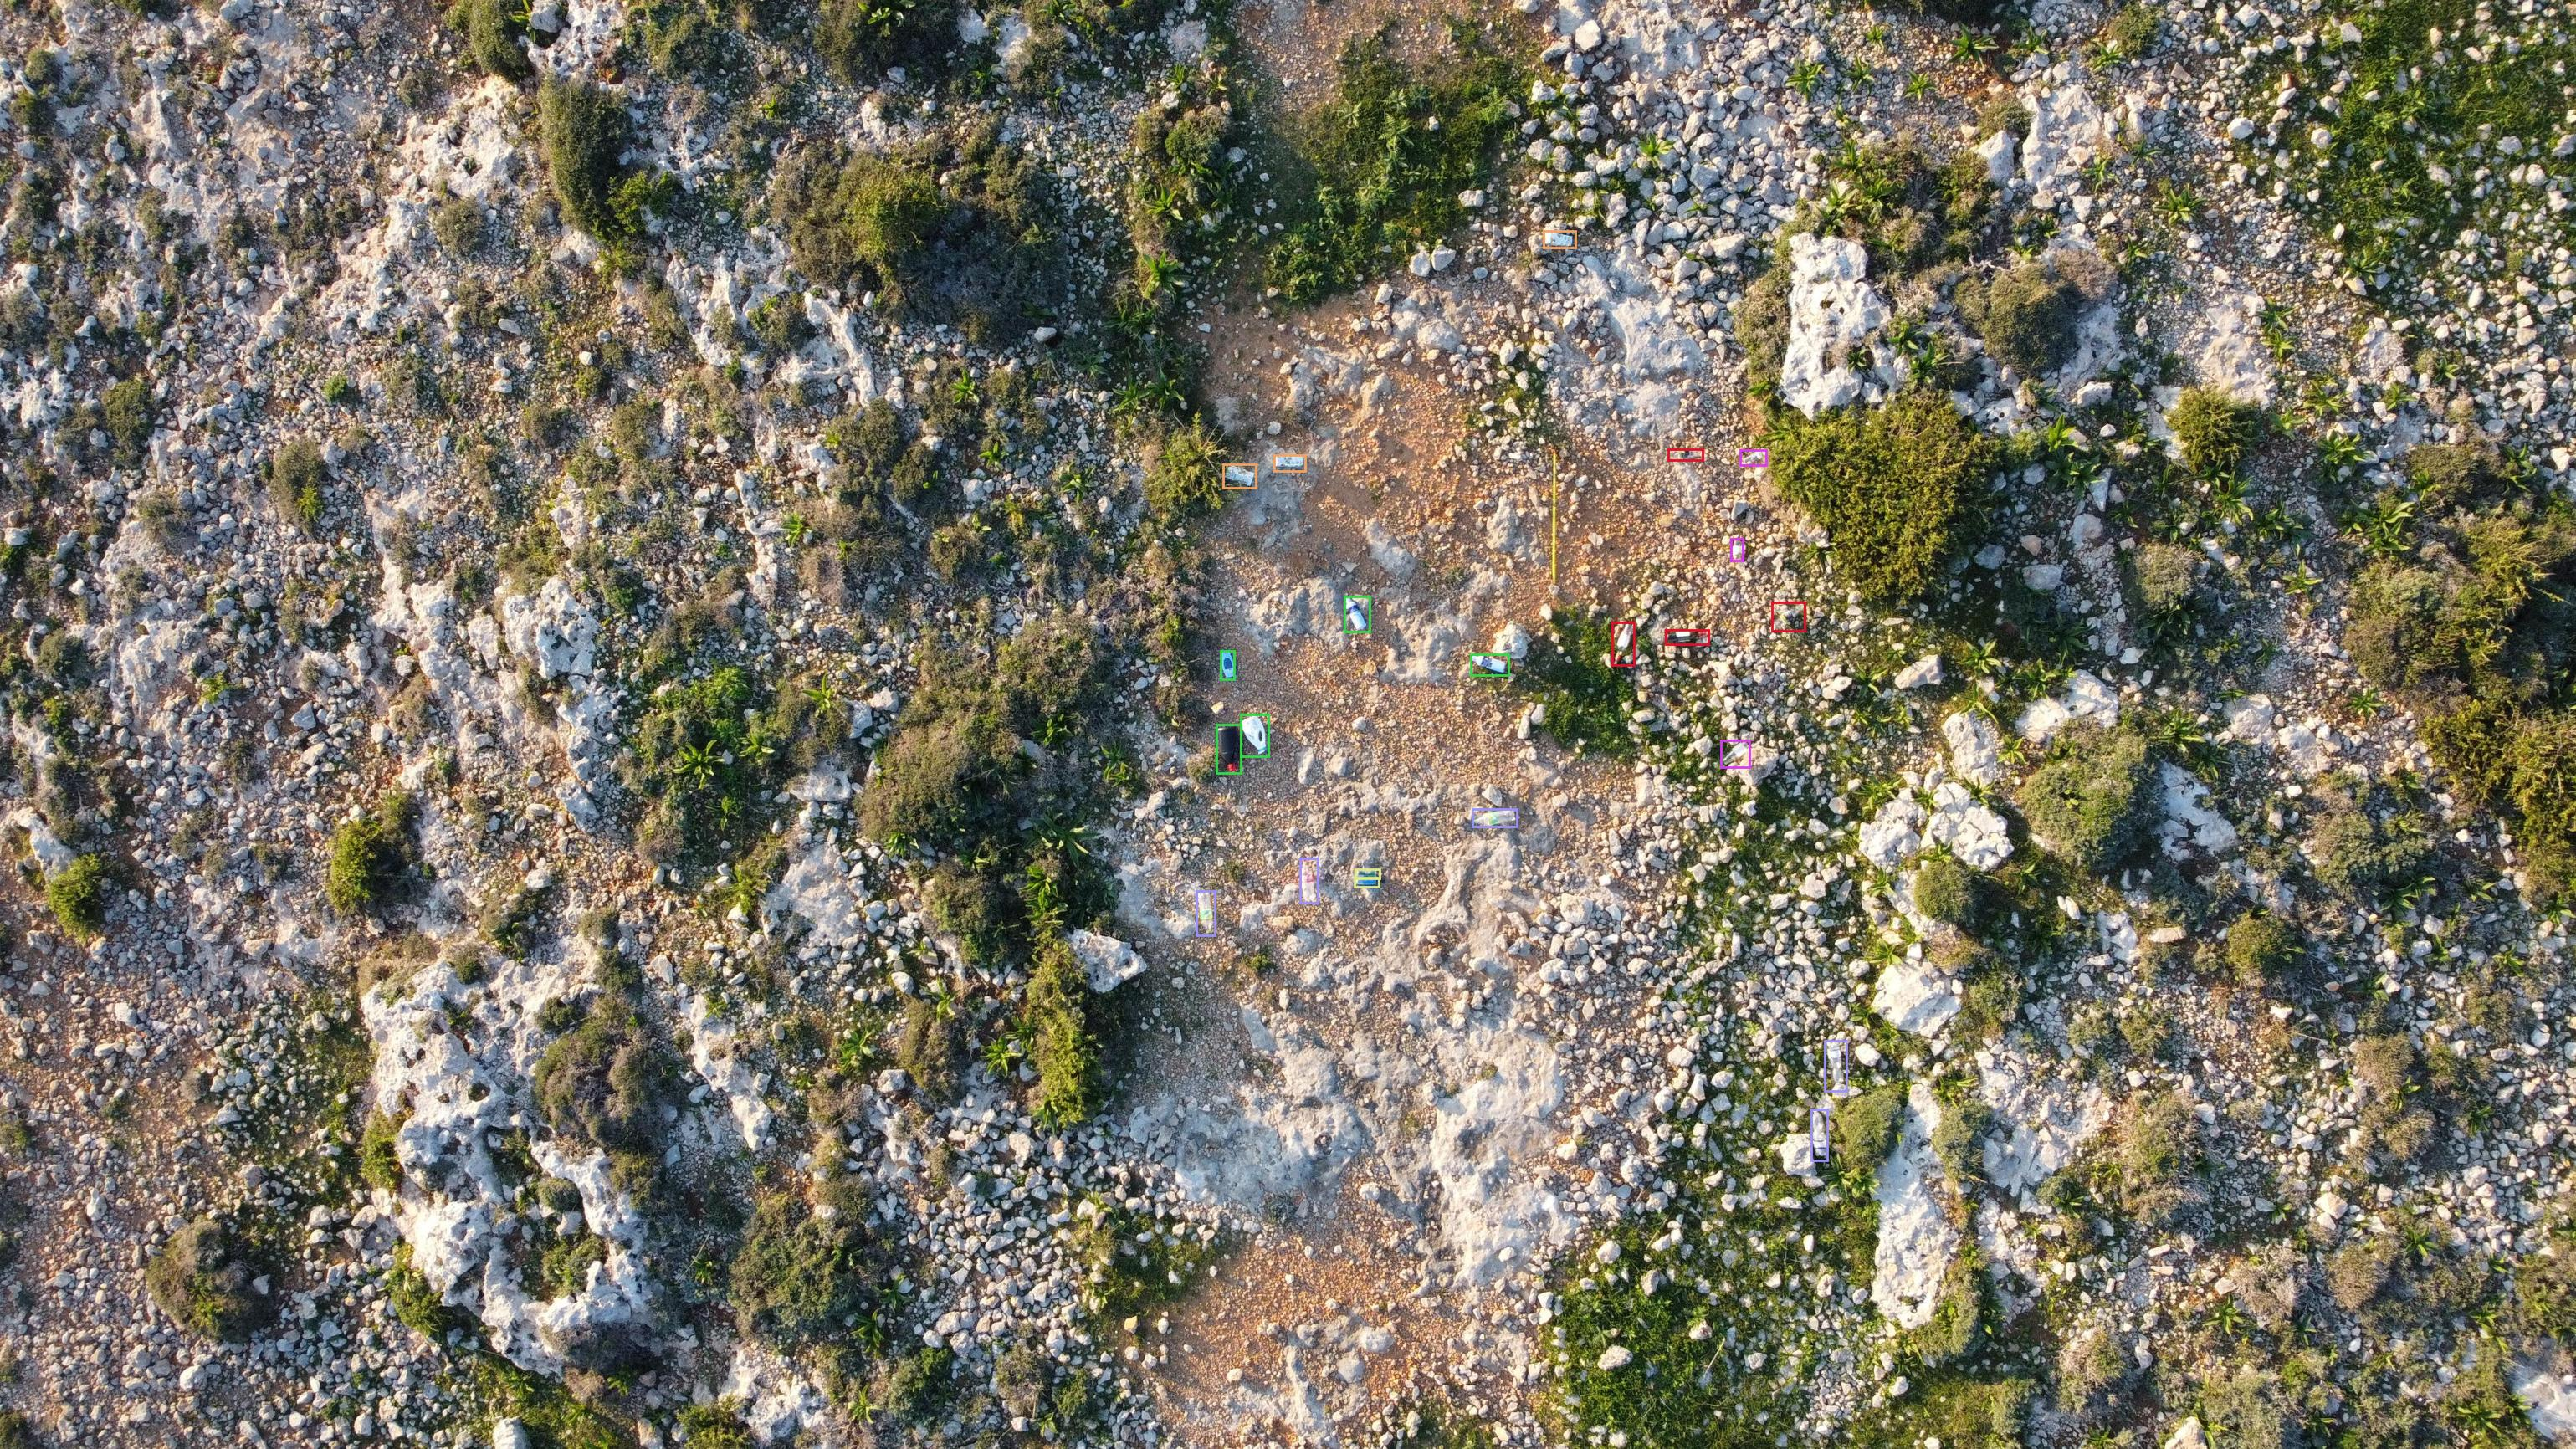
\includegraphics[width=0.98\textwidth]{tiling1.jpg} \\
  \small (a)

  \vspace{1em}

  % Second row of two images
  \begin{tabular}{cc}
    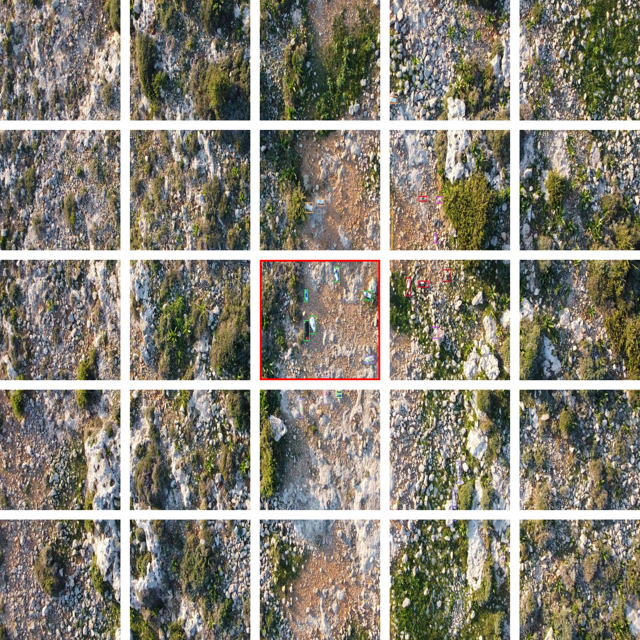
\includegraphics[width=0.48\textwidth, height=4.5cm]{tiling2.png} &
    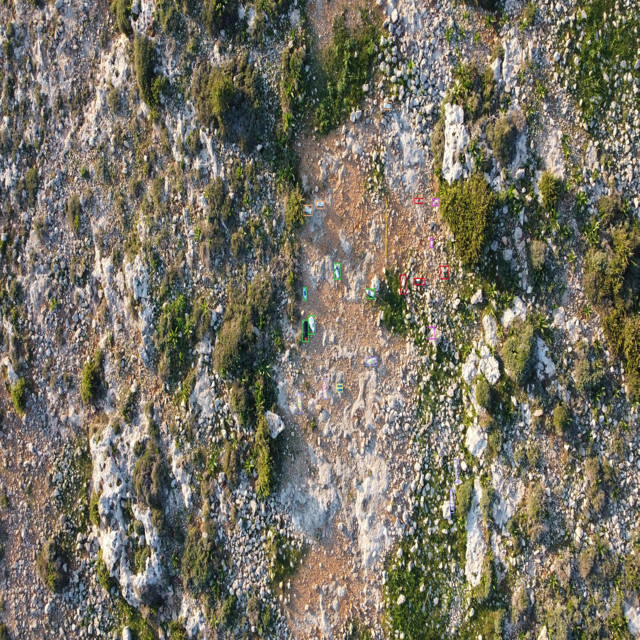
\includegraphics[width=0.48\textwidth, height=4.5cm]{tiling3.png} \\
    \small (b) & \small (c) \\
  \end{tabular}

  \vspace{1em}

  % Third row of two images
  \begin{tabular}{cc}
    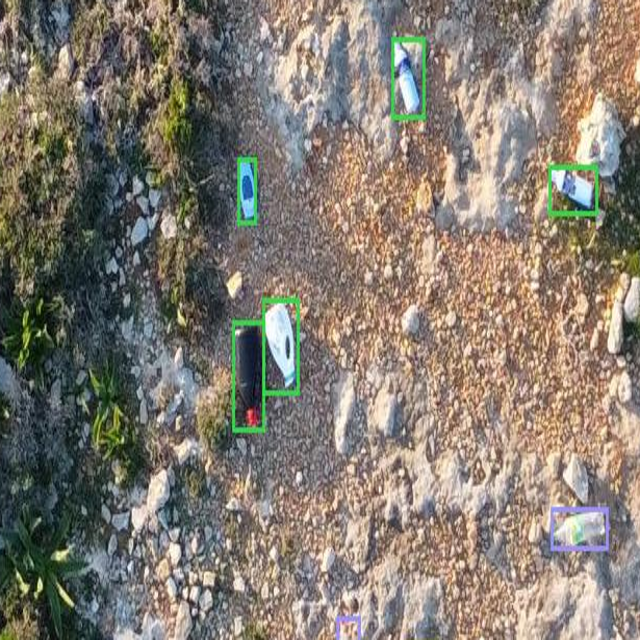
\includegraphics[width=0.48\textwidth, height=4.5cm]{tiling4.png} &
    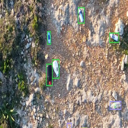
\includegraphics[width=0.48\textwidth, height=4.5cm]{tiling5.png} \\
    \small (d) & \small (e) \\
  \end{tabular}

  \caption{Visual illustration highlighting the need for tiling. (a) Annotated image of litter captured at 15 metres altitude from the SODA dataset \cite{soda_dataset}; (b) 5$\times$5 tiling of the original image, with each tile resized to 640$\times$640 pixels; (c) original image resized directly to 640$\times$640 pixels; (d) the 13\textsuperscript{th} tile from the tiling approach, resized; (e) the corresponding region extracted from the non-tiled image.}

  \label{fig:tiling_examples}
\end{figure}

To understand why such an approach becomes necessary, visual exploration of the data proves useful. Figure \ref{fig:tiling_examples} illustrates this clearly. Subfigure (a) presents an annotated image captured at 15 metres altitude, which is half the maximum altitude in the dataset. If the entire image is resized directly to 640$\times$640 pixels without tiling, as shown in subfigure (c), the result is a significant loss in feature detail. This version represents the full image as it would be input to the detection network in one pass.
Applying tiling, shown in subfigure (b), divides the original image into smaller sections. For example, the 13th tile--resized and displayed in subfigure (d)--shows litter with greater clarity and scale. This makes detection of litter from \gls{uav} footage easier. A side-by-side comparison with the corresponding region from the non-tiled image (subfigure (e)) highlights the reduction in granularity that occurs without tiling.
However, this improved resolution comes at the cost of longer inference times \cite{tiling}, since the model must process several images rather than one. As a result, selecting appropriate tiling parameters involves balancing detection accuracy with computational efficiency.

% Dataset Statistics
For this study, a 3$\times$3 grid was used to tile the \gls{soda} dataset. This choice is supported by the experimental findings discussed in Section \ref{sec:5_tiling_exp}. Additionally, a resize dimension of 800 pixels was applied, based on the rationale presented in Subsection \ref{sec:4_preprocessing}. As a result, the total number of images and annotations increased substantially. The original version of the \gls{soda} dataset contained 829 images. After tiling, this figure rose to 7,461. The image distribution across the category split is presented in Figure~\ref{fig:soda_image_distribution}. Notably, despite the application of these pre-processing steps, the original ratio between the training, validation, and testing sets remains consistent before and after tiling.
\begin{figure}[!ht]
  \centering
  \begin{tabular}{c}
    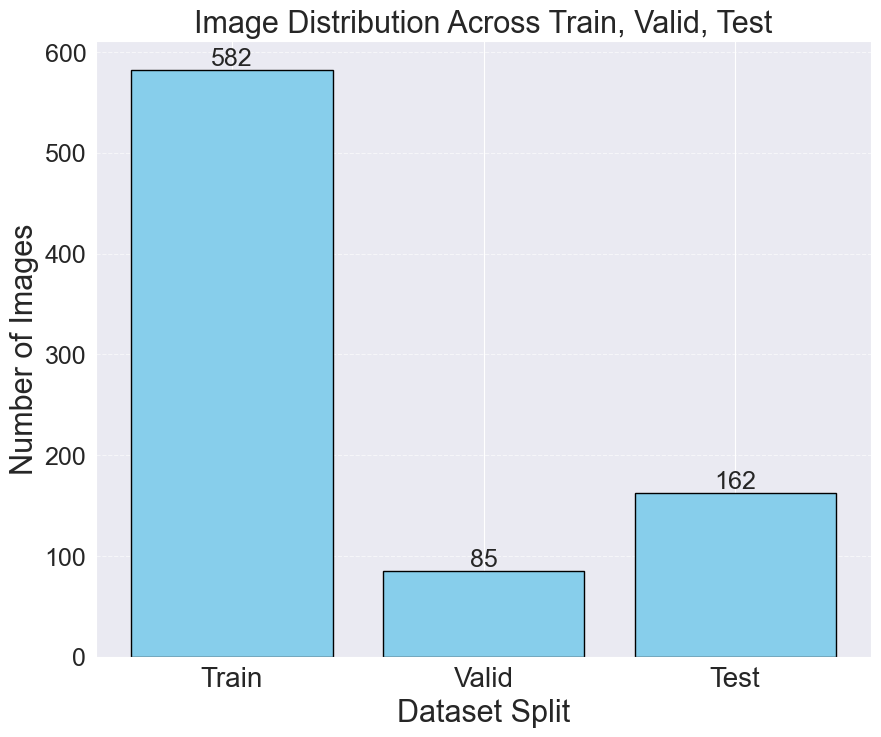
\includegraphics[width=0.6\textwidth]{image_distribution1.png} \\
    \small (a) \\
    \addlinespace[1em]
    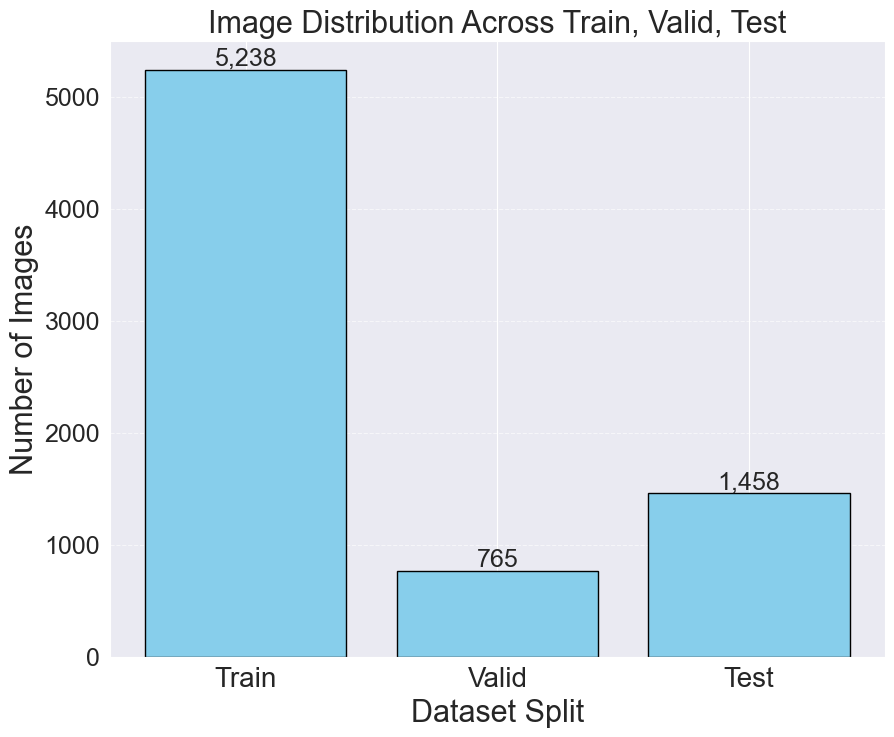
\includegraphics[width=0.6\textwidth]{image_distribution2.png} \\
    \small (b) \\
  \end{tabular}
  \caption{\gls{soda} dataset image distribution: (a) before 3$\times$3 tiling, and (b) after 3$\times$3 tiling.}
  \label{fig:soda_image_distribution}
\end{figure}

Additionally, with the use of tiling, the spatial distribution of object annotations changed significantly. As the number of images increased, the objects became larger and more defined, helping to mitigate the annotation bias present in the original \gls{soda} dataset. This is illustrated in Figure~\ref{fig:soda_annotation_heatmap}. In subfigure (a), the heatmap before tiling shows a strong centre bias. After tiling, shown in subfigure (b), this bias is less pronounced, with a more even distribution across the heatmap, though some focus on the centre remains. The pixel intensities also increased due to the larger number of images and annotations.

\begin{figure}[!ht]
  \centering
  \begin{tabular}{c}
    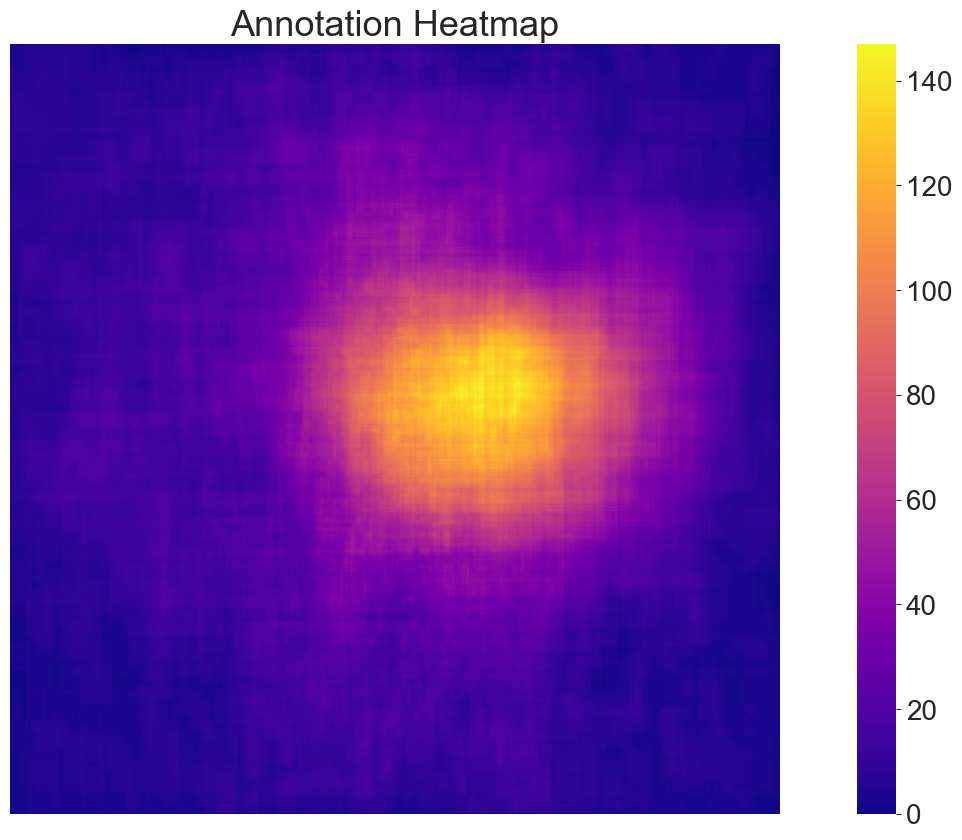
\includegraphics[width=0.6\textwidth]{annotation_heatmap1.png} \\
    \small (a) \\
    \addlinespace[1em]
    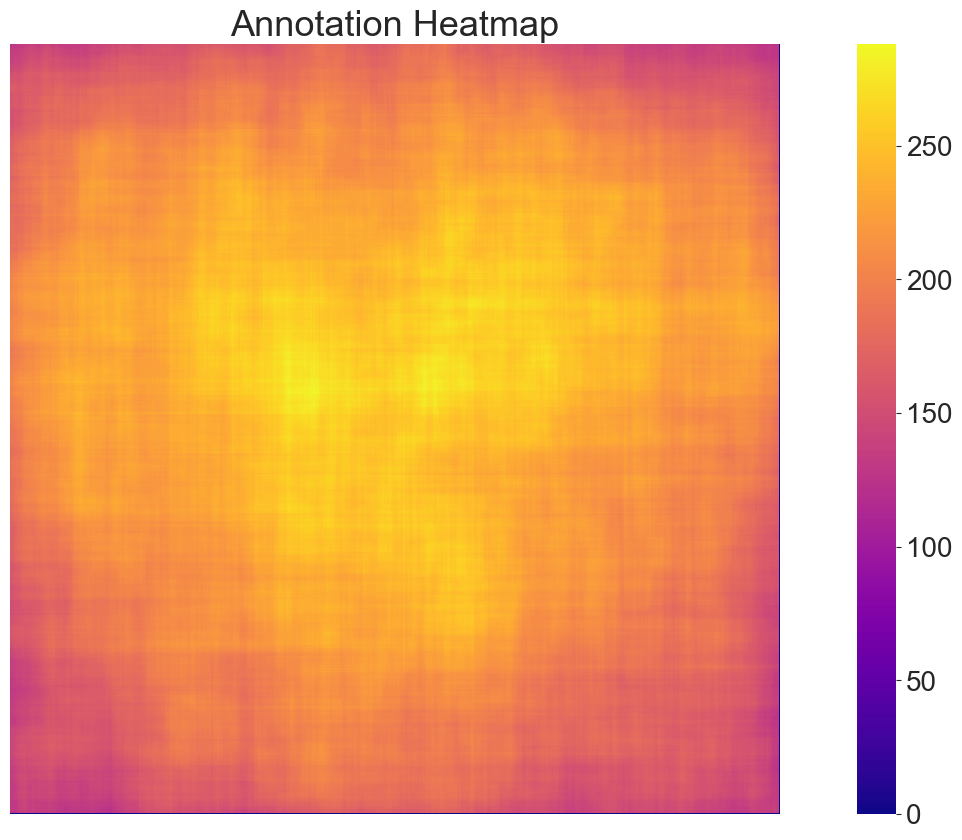
\includegraphics[width=0.6\textwidth]{annotation_heatmap2.png} \\
    \small (b) \\
  \end{tabular}
  \caption{\gls{soda} dataset annotation heatmap: (a) before 3$\times$3 tiling, and (b) after 3$\times$3 tiling.}
  \label{fig:soda_annotation_heatmap}
\end{figure}

Tiling unintentionally worsened the class imbalance. As images were split into smaller sections, some object bounding boxes were also divided. This was especially the case for objects near the edges or those covering a larger area. Common categories like \textit{Drink Can} and \textit{Clear Plastic Bottle}, which were already more frequent, appeared even more often after tiling. This shift is reflected in the category distribution shown in Figure \ref{fig:soda_annotation_distribution}.
Meanwhile, less frequent classes such as \textit{Glass Jar} and \textit{Drink Carton} showed a marginal increase in representation. Interestingly, \textit{Glass Bottle} surpassed Other \textit{Plastic Bottle} in the number of annotations, reversing their relative frequencies before tiling.

\begin{figure}[!ht]
  \centering
  \begin{tabular}{c}
    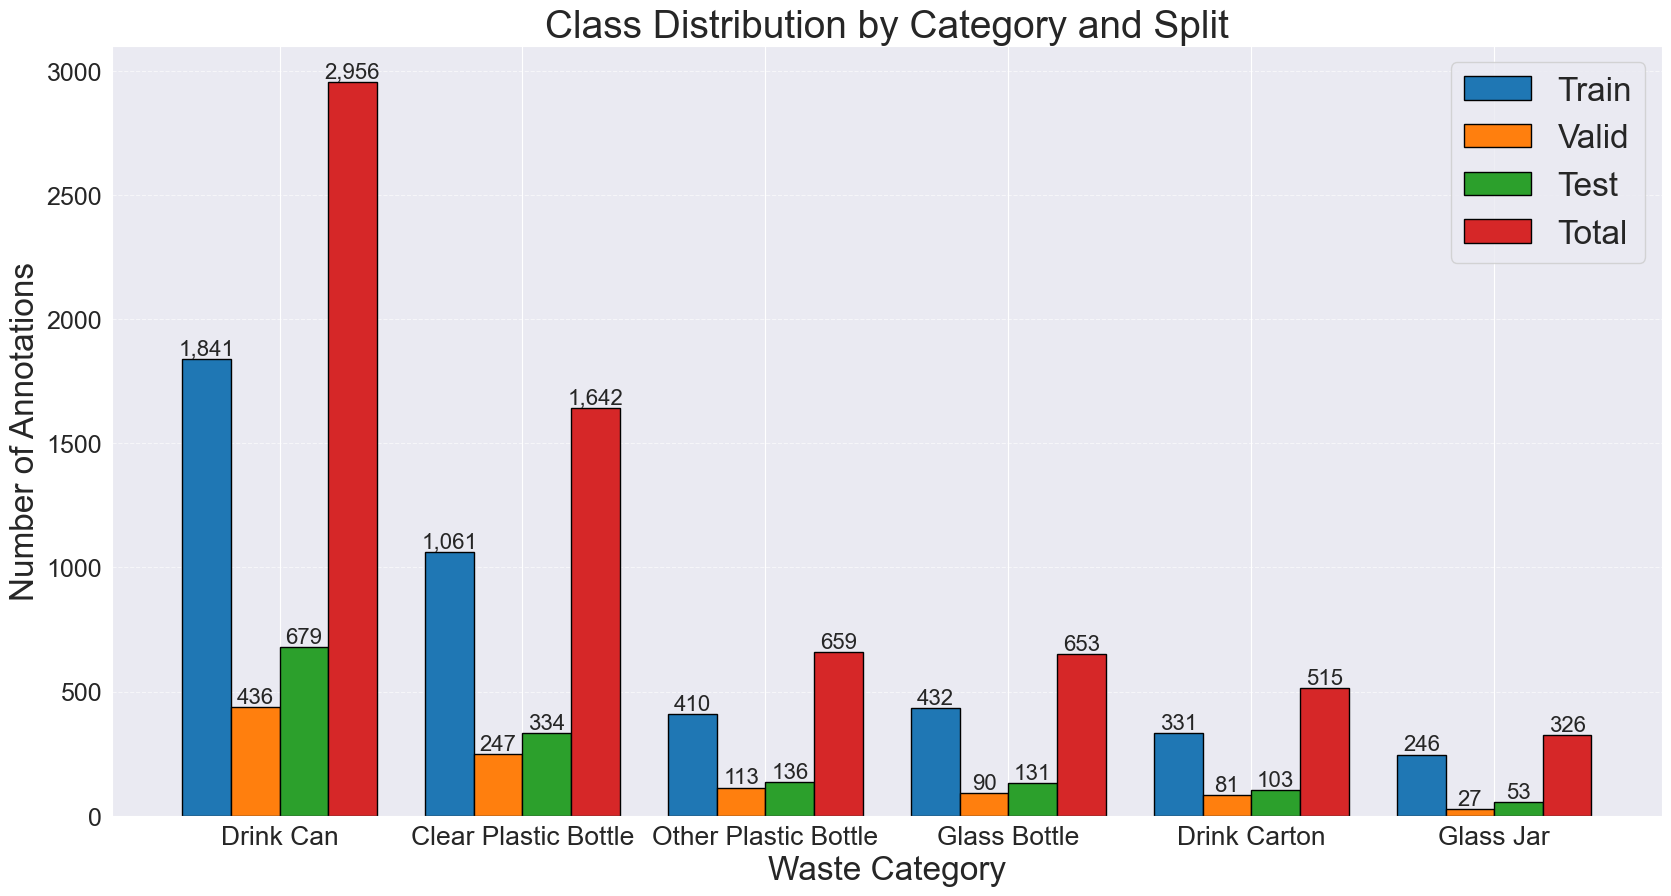
\includegraphics[width=1\textwidth]{annotation_distribution1.png} \\
    \small (a) \\
    \addlinespace[1em]
    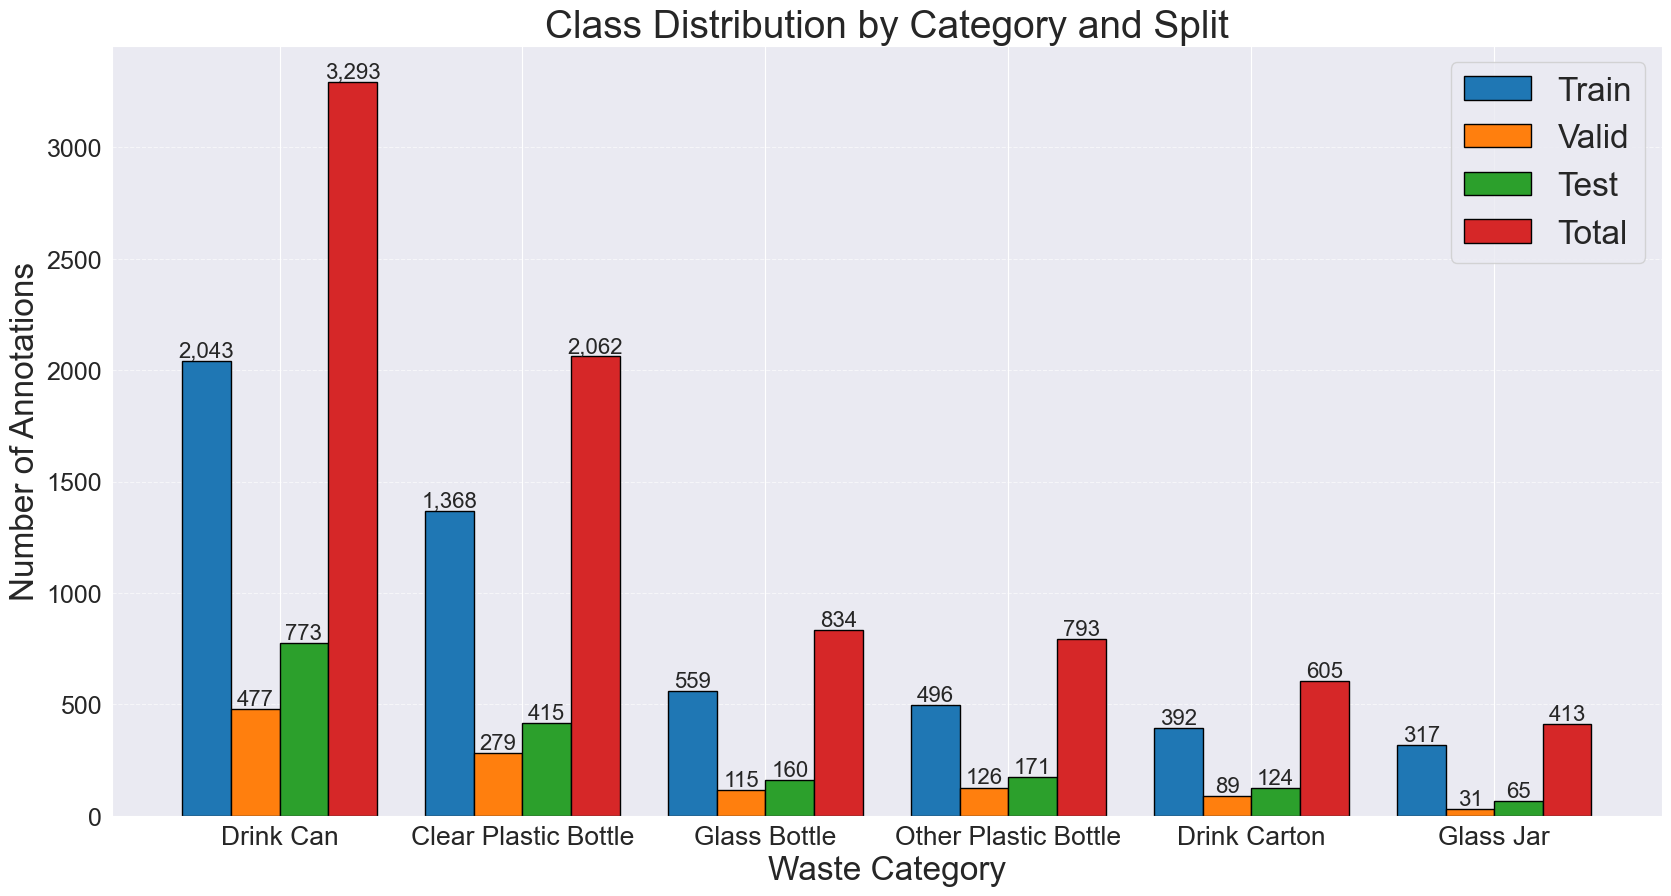
\includegraphics[width=1\textwidth]{annotation_distribution2.png} \\
    \small (b) \\
  \end{tabular}
  \caption{\gls{soda} dataset annotation distribution per category and split: (a) before 3$\times$3 tiling, and (b) after 3$\times$3 tiling.}
  \label{fig:soda_annotation_distribution}
\end{figure}

The increase in annotations due to tiling has had a significant impact on the overall distribution of object sizes. Using the object size classifications from the \gls{coco} dataset \cite{coco}, where objects are defined as small (less than 32$\times$32 pixels), medium (ranging from 32$\times$32 to 96$\times$96 pixels), and large (greater than 96$\times$96 pixels), a clear shift in object size distribution can be observed. As shown in Figure~\ref{fig:soda_object_size_distribution}, while the total number of objects has increased, the proportion of small objects has decreased, with a corresponding rise in both medium and large objects. This shift in distribution suggests an improvement in the dataset’s size balance, which should improve the detection of previously smaller objects. With the larger objects now more prominent, the detection models can benefit from improved size constraints, making these objects easier to detect.

% \clearpage

\begin{figure}[!ht]% Values taken from TIling Experiment which was more reliable
  \centering
  \begin{tabular}{c}
    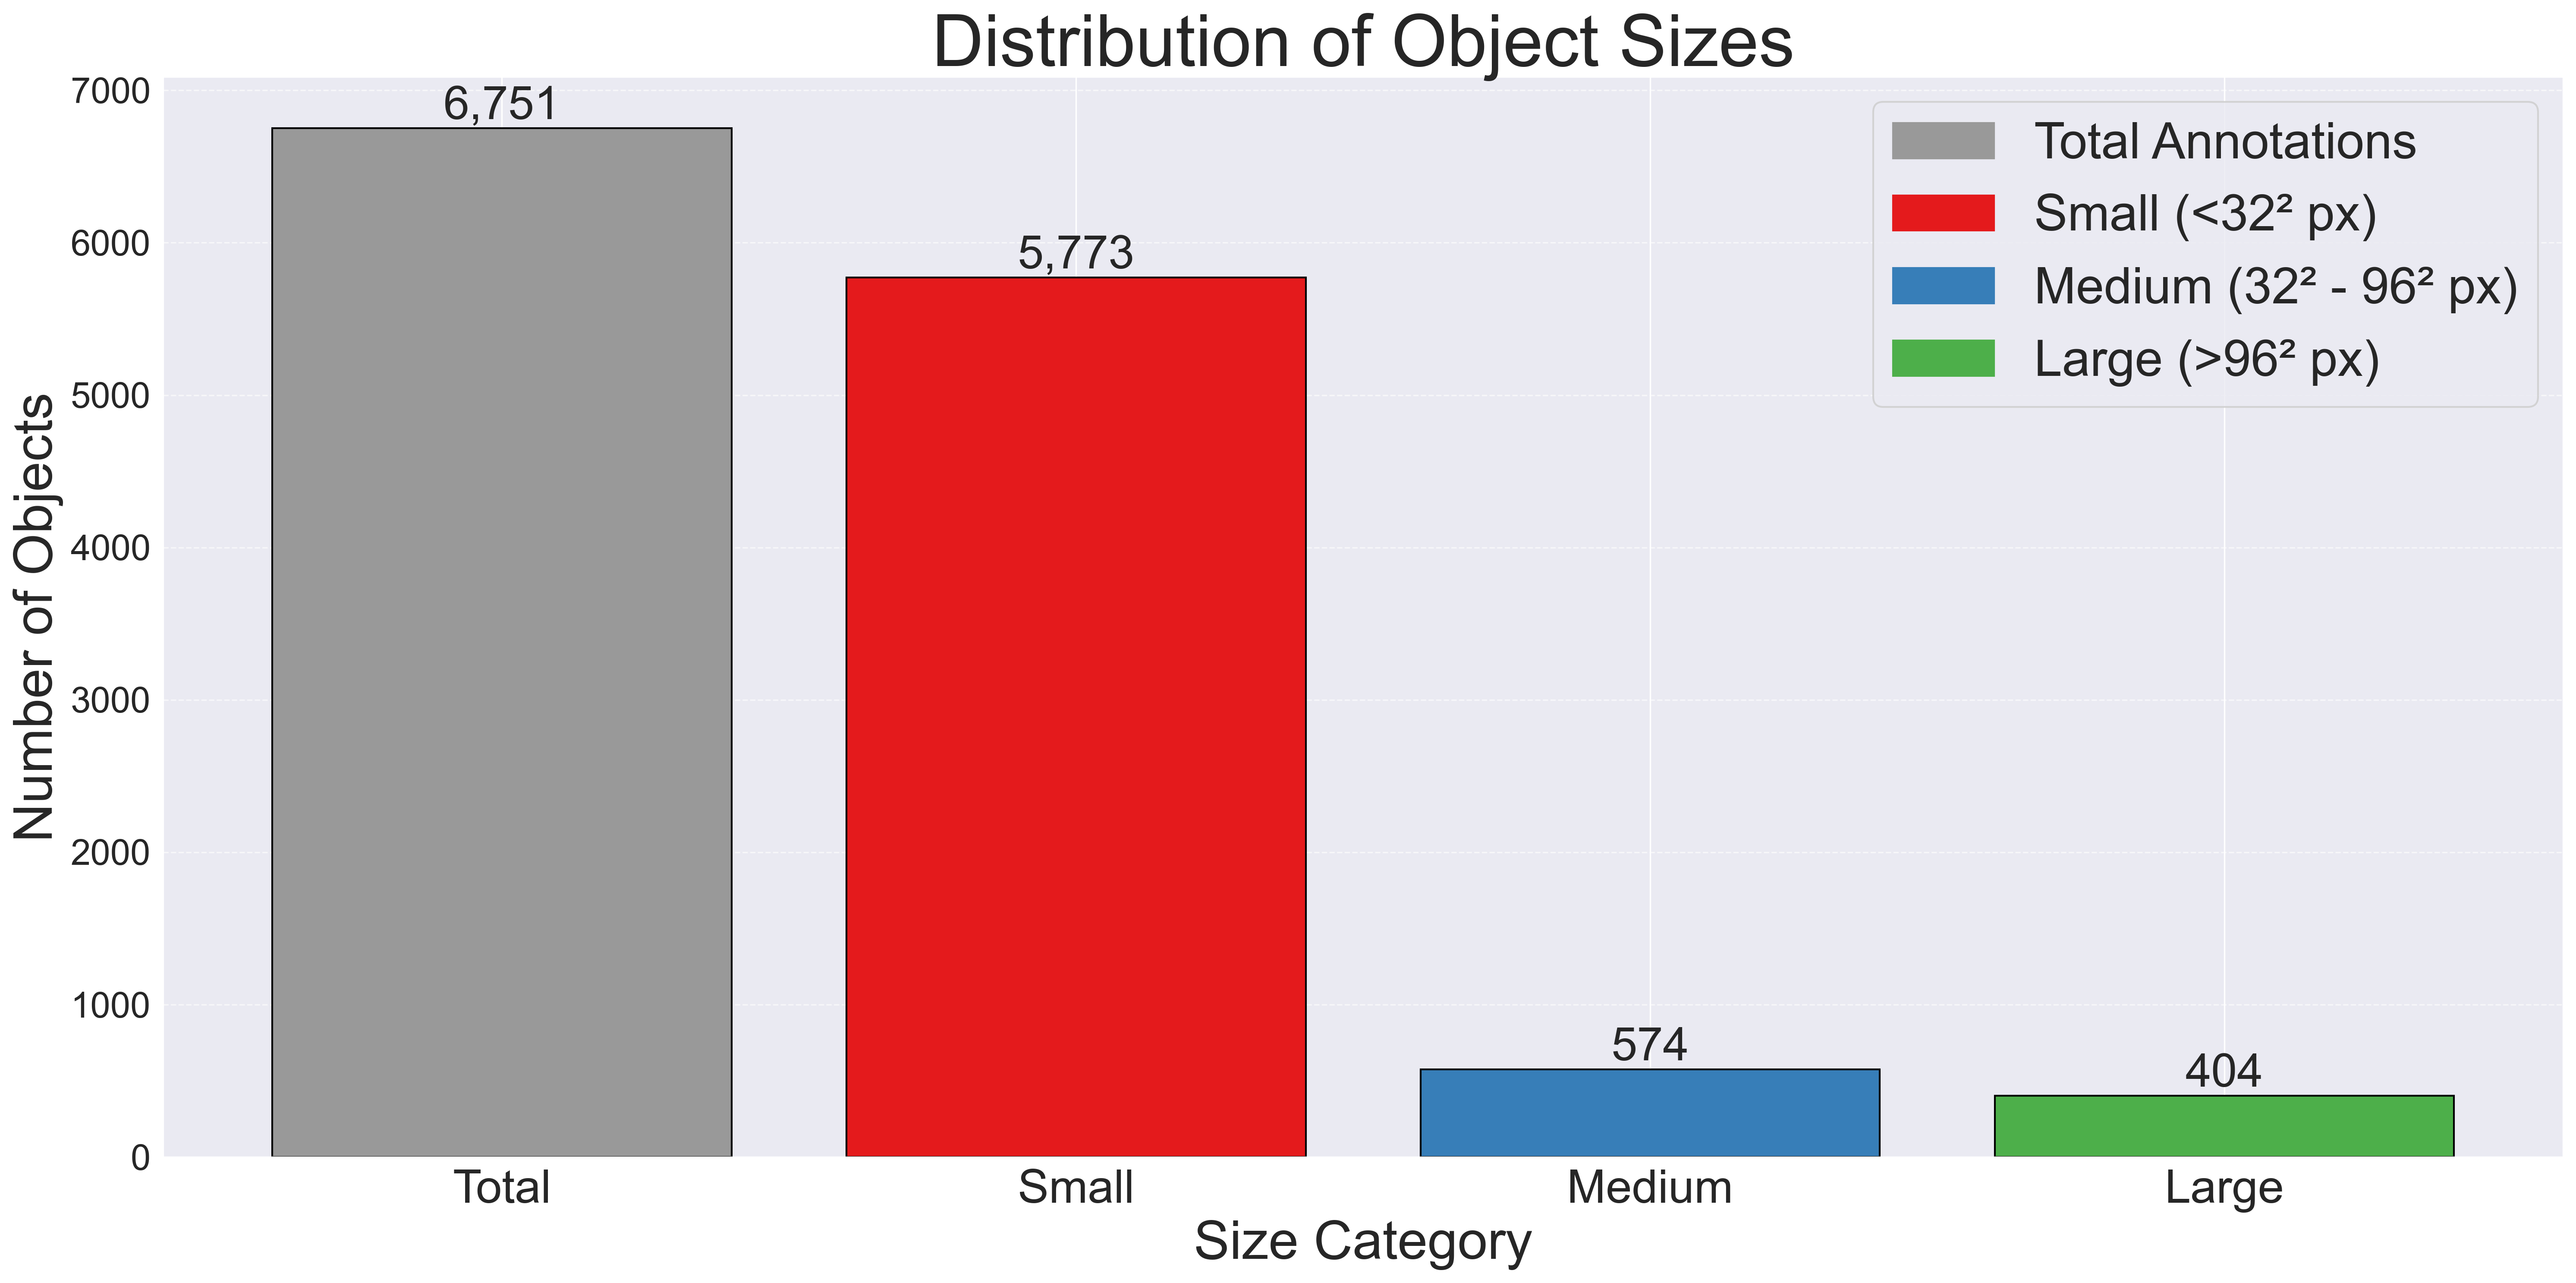
\includegraphics[width=0.9\textwidth]{object_size_distribution1.png} \\
    \small (a) \\
    \addlinespace[1em]
    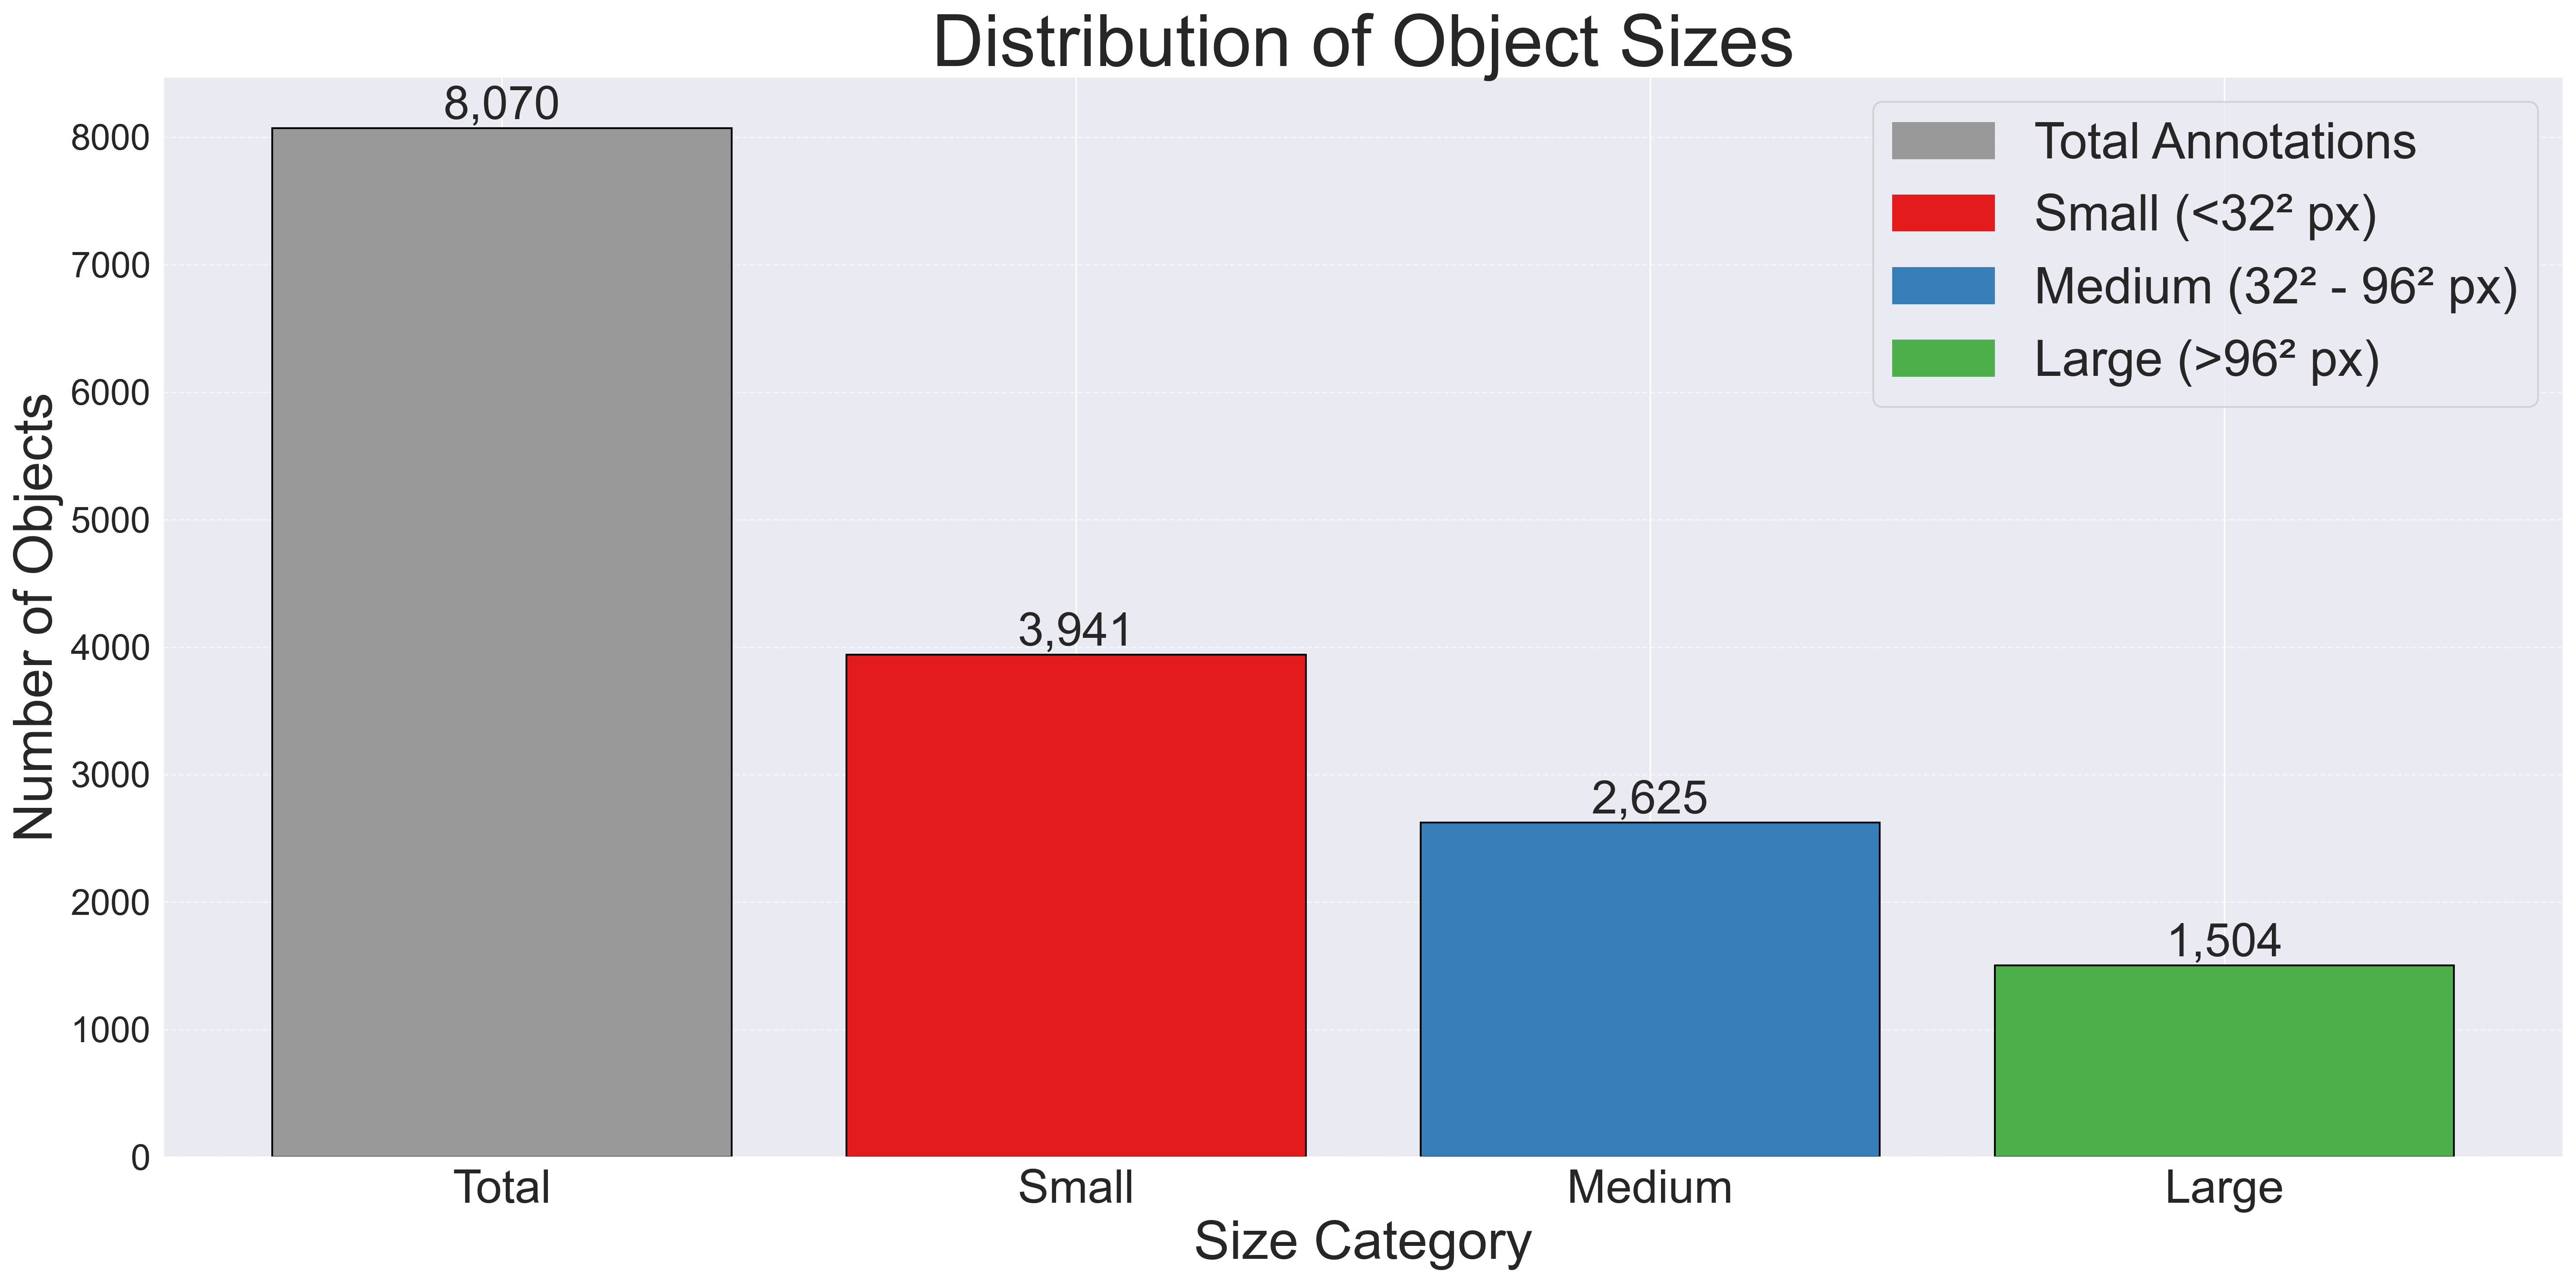
\includegraphics[width=0.9\textwidth]{object_size_distribution2.png} \\
    \small (b) \\
  \end{tabular}
  \caption{\gls{soda} dataset object size distribution: (a) before 3$\times$3 tiling, and (b) after 3$\times$3 tiling.}
  \label{fig:soda_object_size_distribution}
\end{figure}

In summary, tiling has proven to be quite beneficial in improving the detection of objects in the \gls{soda} dataset, particularly for smaller objects. While it helped reduce some of the bias in annotations, it also introduced new challenges, especially regarding class imbalance. This tiling setup has been utilised to magnify and address the issue of small litter detection for the chosen case study, which will be used in the experiments discussed in Section \ref{sec:5_within_dataset_exp}.


\subsection{BDW: Bottle Detection in the Wild}
\label{subsec:4_bdw}

The \gls{bdw} dataset \cite{bdwdataset}, mentioned in Subsection \ref{subsec:3_bdw}, contains 25,407 images taken at altitudes between 10 and 30 metres, but it focuses only on detecting bottles. For this study, this dataset will be used solely for evaluation, as it only covers the representation of bottles, thus limiting the generalisability of the results. Therefore, only the testing set, consisting of 5,078 images, will be used to evaluate the models. Although the dataset claims to include images captured at higher altitudes, the objects in these images, as shown in Figure \ref{fig:bdw_samples}, appear relatively large and clear. This suggests that an image-splitting technique may have been applied during data collection.

\begin{figure}[!htbp]
  \centering
  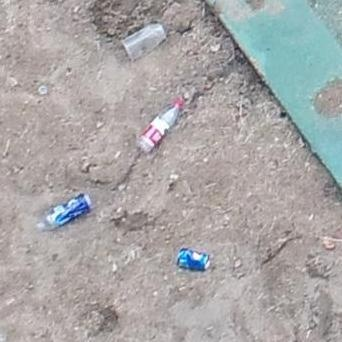
\includegraphics[width=0.32\textwidth]{bdw1.jpg}
  \hfill
  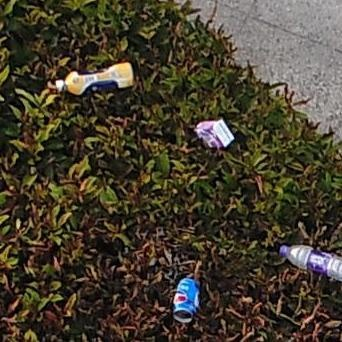
\includegraphics[width=0.32\textwidth]{bdw2.jpg}
  \hfill
  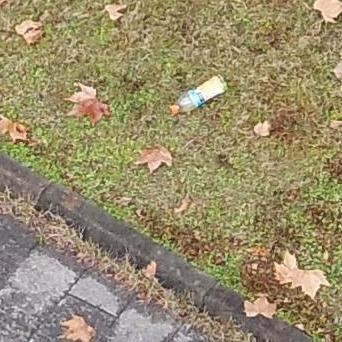
\includegraphics[width=0.32\textwidth]{bdw3.jpg}
  \caption{Sample images from the test subset of the \gls{bdw} dataset, illustrating the general nature of the data. (Source: \cite{bdwdataset})}
  \label{fig:bdw_samples}
\end{figure}


\subsection{UAVVaste}
\label{subsec:4_uavvaste}

UAVVaste \cite{uavvaste}, the final publicly available \gls{uav}-based litter detection dataset chosen for this study, and as discussed in Subsection \ref{subsec:3_uavvaste}, contains 772 images captured at unspecified low altitudes, with various forms of litter annotated under a single waste category. In this study, the dataset will be used exclusively for evaluation, as its focus on low-altitude imagery limits generalisation. Only the testing set, containing 77 images, will be used to evaluate the trained models. A visual inspection of the dataset, as shown in Figure \ref{fig:uavvaste_samples}, suggests the images were likely captured at altitudes between 5 and 10 metres \gls{agl}.

\begin{figure}[!htbp]
  \centering
  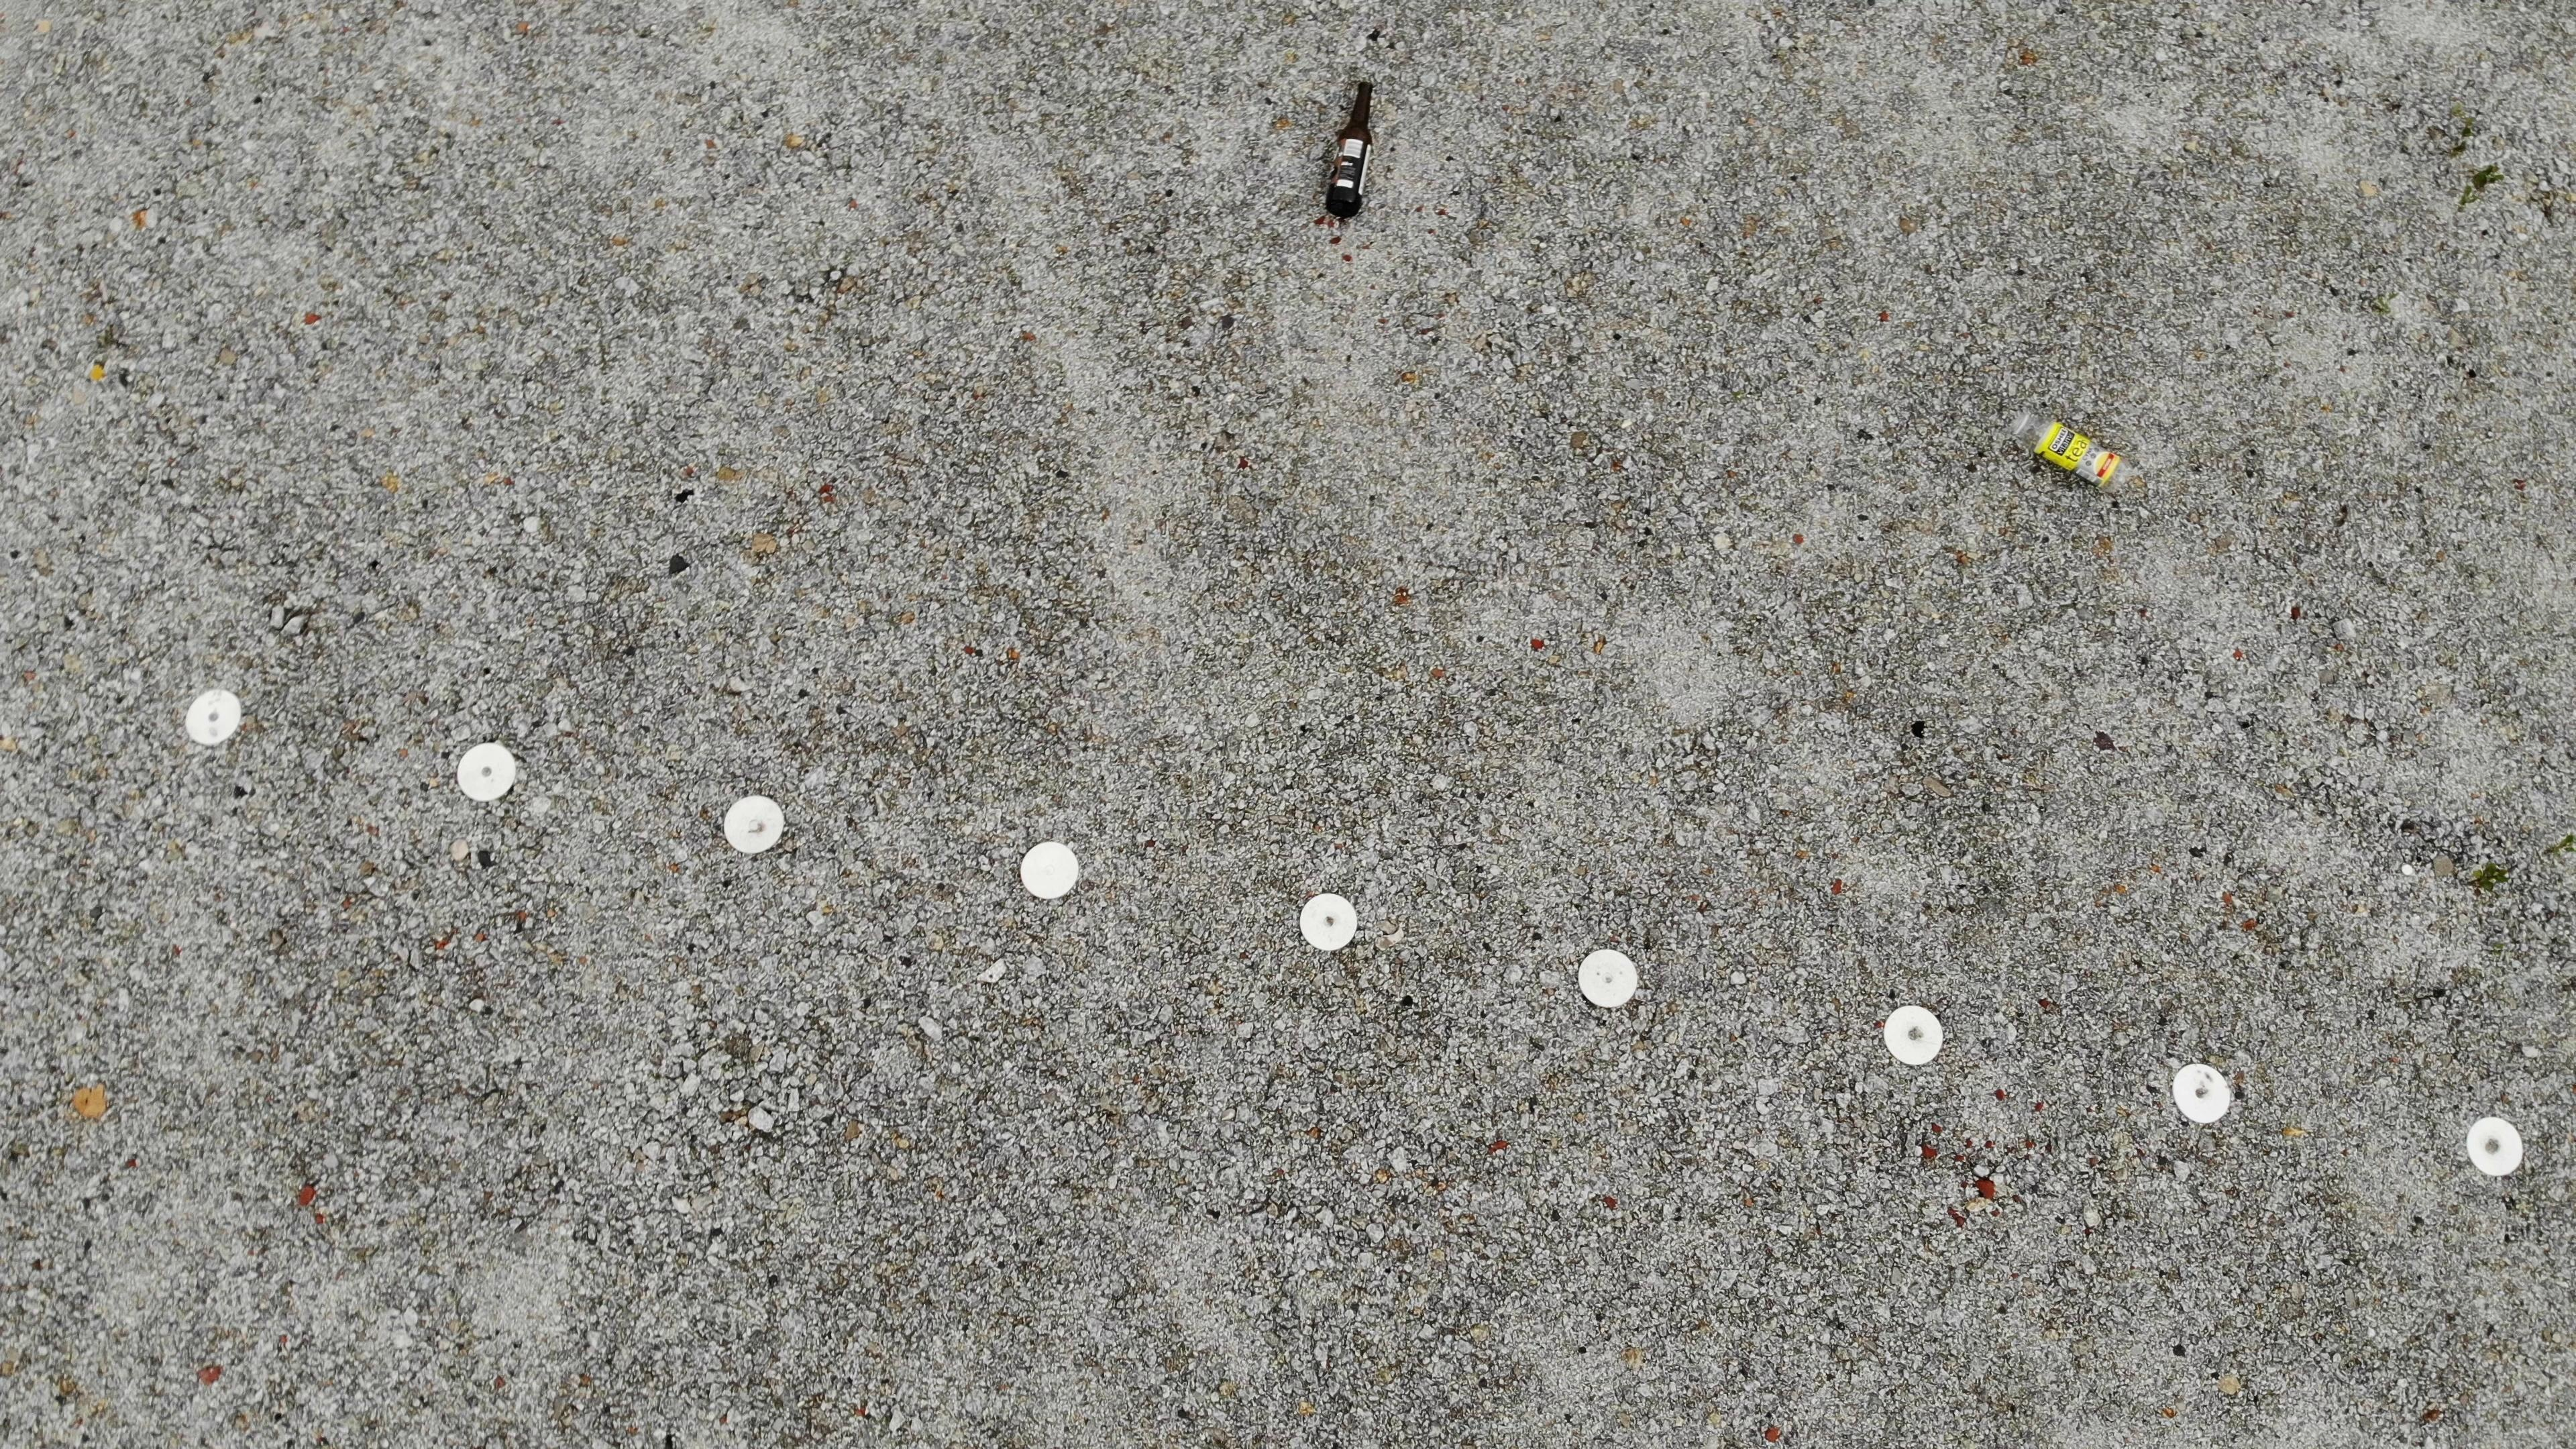
\includegraphics[width=0.48\textwidth]{uavvaste1.jpg}
  \hfill
  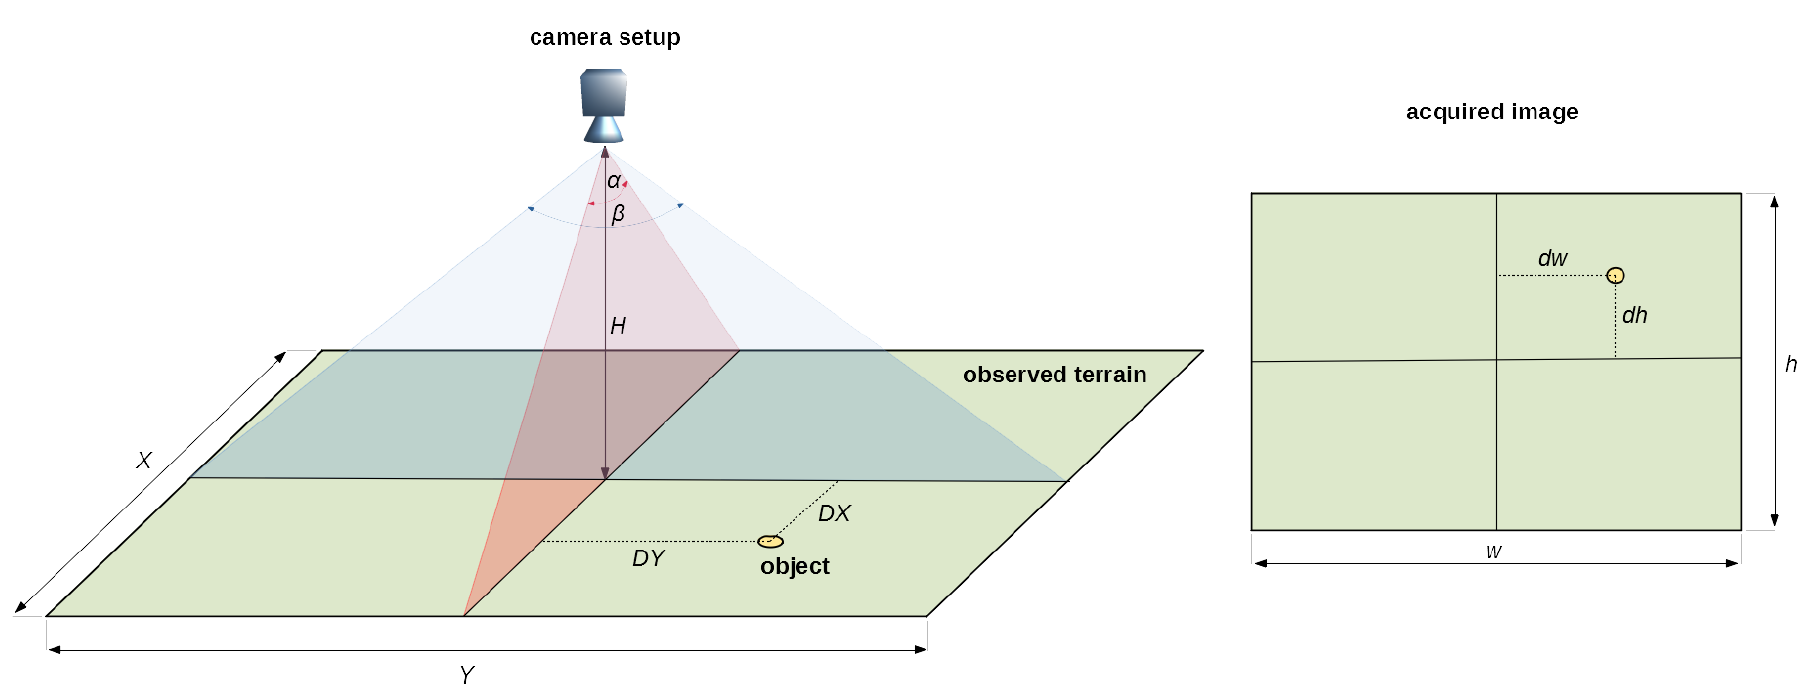
\includegraphics[width=0.48\textwidth]{uavvaste2.jpg}
  \caption{Sample images from the test subset of the UAVVaste dataset, illustrating the general nature of the data. (Source: \cite{uavvaste})}
  \label{fig:uavvaste_samples}
\end{figure}


\subsection{Pascal Visual Object Classes}
\label{subsec:4_pascal_voc}

Pascal \gls{voc} is a widely used benchmark dataset in object detection, featuring 20 object categories including people, animals, vehicles, and various household items \cite{pascal-voc-2012}. Figure \ref{fig:pascal_voc} shows sample images that illustrate the diversity of the dataset. The dataset includes images annotated with object class labels, bounding boxes, and pixel-level segmentation masks, enabling its use across multiple computer vision tasks. In this study, the Pascal \gls{voc} 2012 dataset is used for both training and validation to test the proposed methodology beyond the context of \gls{uav}-based litter detection, per the fourth objective (\textbf{O4}). This helps assess whether the approach remains effective across a broader set of object classes. 

\begin{figure}[!htbp]
    \centering
    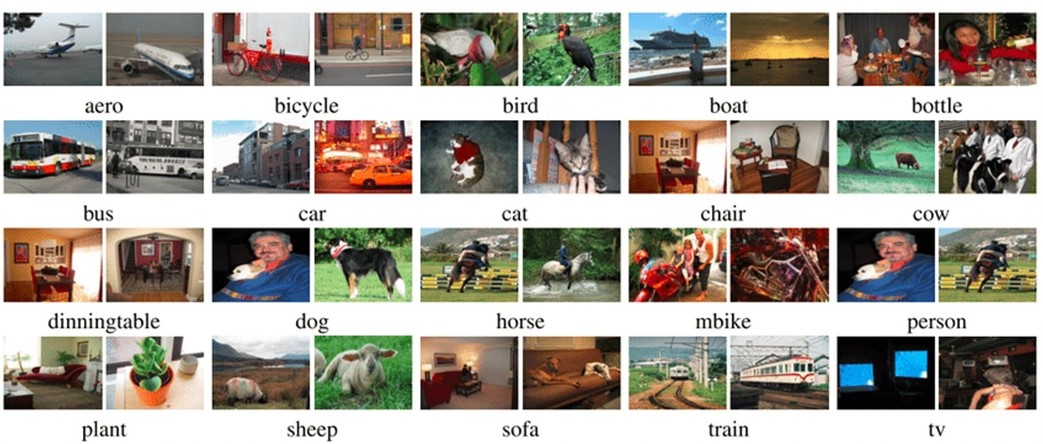
\includegraphics[width=1\textwidth]{pascalvoc2012images.jpg}
    \caption{Sample images from the Pascal VOC 2012 dataset, showcasing the diversity in object categories included in the dataset. (Source: \cite{pascal-voc-2012})}
    \label{fig:pascal_voc}% Resized to 200%
\end{figure}

The dataset utilised in this study, sourced from Roboflow, contains 17,112 images in total. Of these, 13,690 are assigned to the training set, and 3,422 are designated for validation. However, the Pascal VOC 2012 dataset also suffers from class imbalance, as shown in Figure~\ref{fig:class_distribution_pascal_voc}. There is a disproportionately high number of instances labelled as \textit{person} compared to other categories. While the remaining classes show smaller gaps among themselves, class imbalance is still present, with \textit{bus} being the least represented category.

\begin{figure}[!ht]
    \centering
    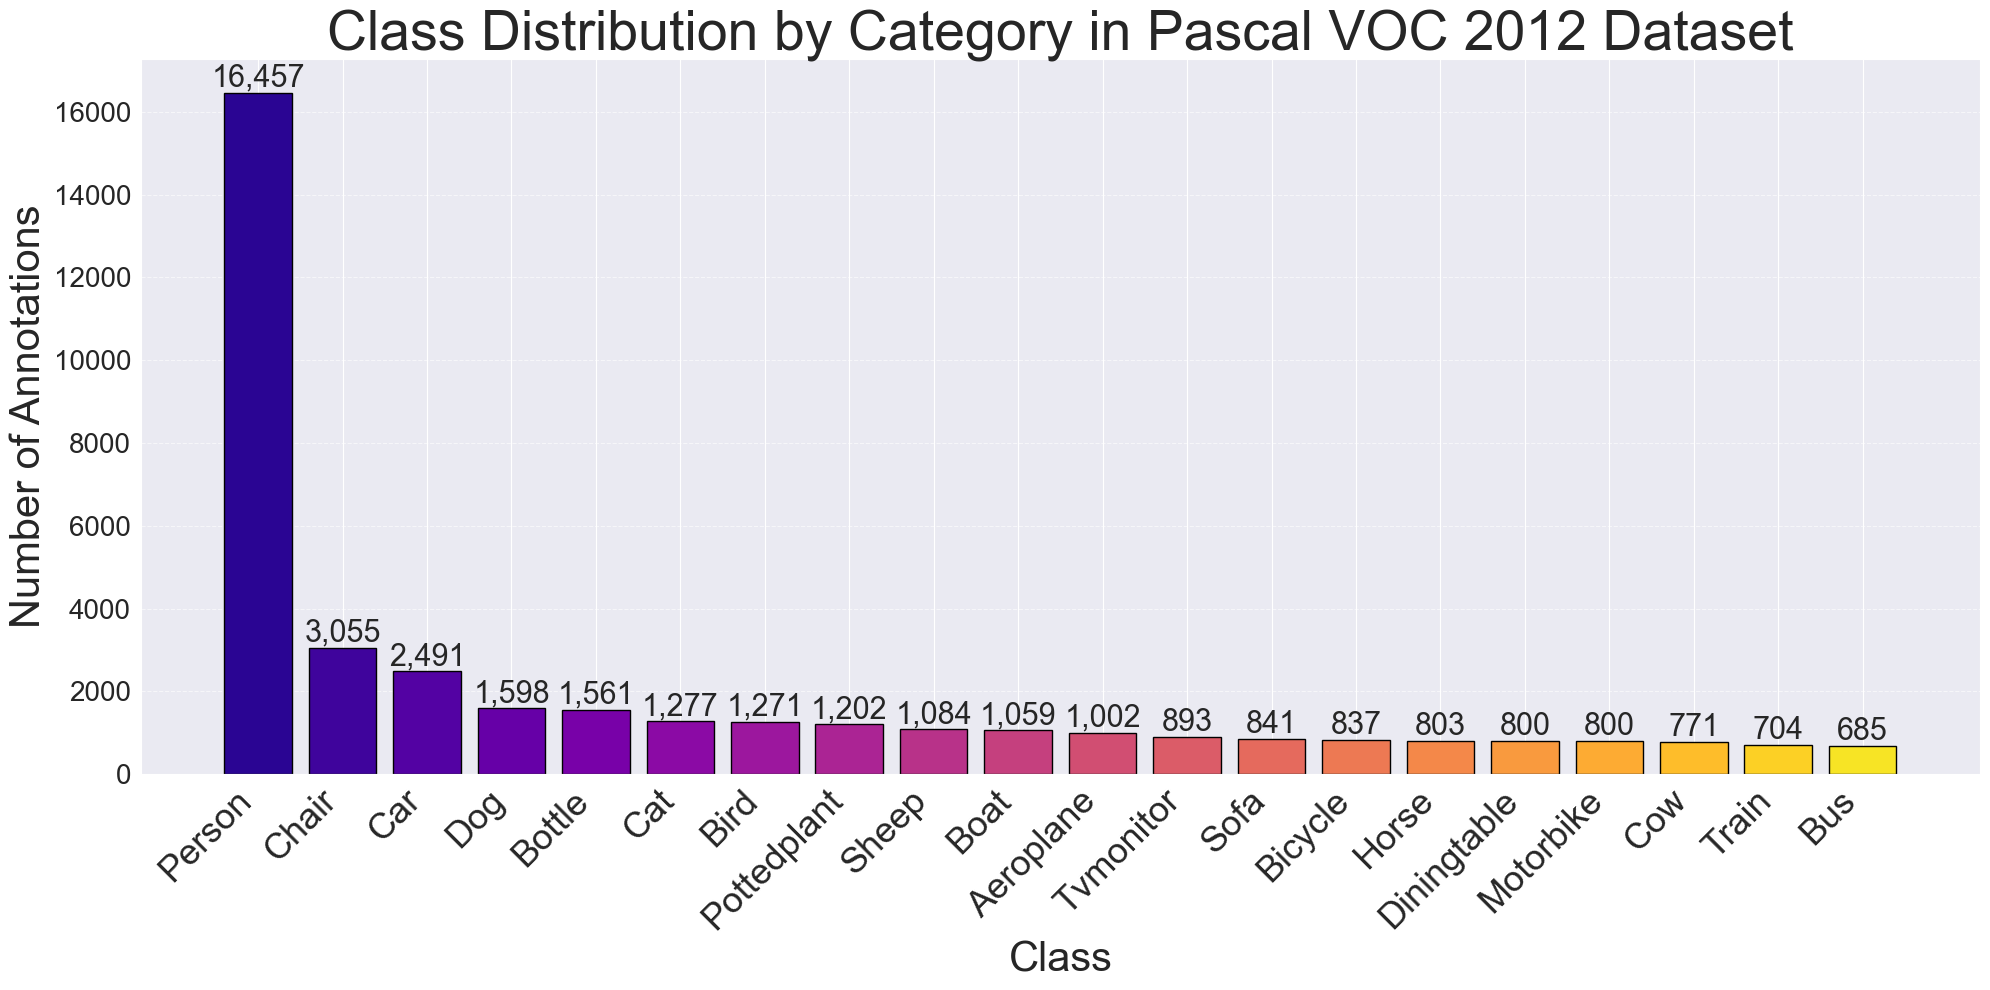
\includegraphics[width=1\textwidth]{annotation_distribution_pascal.png}
    \caption{Class distribution of the Pascal VOC 2012 dataset, highlighting the imbalance across different categories, with the number of objects per class from both the training and validation splits.}
    \label{fig:class_distribution_pascal_voc}% Resized to 200%
\end{figure}

\section{Metrics}
\label{sec:4_metrics}
% Glorja lil Missier, lil-Iben, u lil-Ispirtu s-Santu kif kien mill-bidu issa u dejjem ghal-dejjem. Amen.

Having outlined the importance of datasets and identified those relevant to this study, it is essential to evaluate the quantitative performance of object detection techniques to gauge their effectiveness in addressing the detection problem, in line with objectives \textbf{O2} through \textbf{O4}. The evaluation of these systems primarily involves comparing model predictions (bounding boxes and labels) with ground truth annotations using the Intersection over Union (\gls{iou}) metric, which measures the overlap between predicted and actual bounding boxes. The \gls{iou} threshold determines the minimum overlap needed for a prediction to be considered a true positive. Lower thresholds (e.g., 0.5) allow for more flexible matching, whereas higher thresholds (e.g., 0.75) set stricter criteria \cite{coco}. This metric also facilitates the computation of important evaluation indicators: \gls{tp}, which are correctly identified objects with an \gls{iou} above the threshold; \gls{fp}, which are objects incorrectly identified or those with insufficient overlap; and \gls{fn}, which are objects missed by the model that are present in the ground truth. \gls{tn} are generally not included in object detection evaluations, as they correspond to the correct identification of the absence of an object.

\gls{iou}, or Jaccard’s Index, serves as a metric for evaluating the overlap between the predicted bounding box and the ground truth, offering a quantitative measure of the precision in object localisation. As demonstrated in Equation \ref{eqn:iou}, $b$ denotes the predicted bounding box, while $g$ refers to the ground truth. A higher \gls{iou} value, with a maximum of 1, signifies greater accuracy in the predictions, indicating a smaller deviation between the predicted bounding box and the ground truth.
\begin{equation}
\label{eqn:iou}
\text{IoU}(b, g) = \frac{{\text{area}(b \cap g)}}{{\text{area}(b \cup g)}}.
\end{equation}
Precision, as outlined in Equation \ref{eqn:precision}, measures the proportion of relevant items retrieved by the model. It is determined by the ratio of \gls{tp}, which are objects correctly identified as relevant, to the sum of \gls{tp} and \gls{fp}, which denotes the total number of objects that were mistakenly identified as relevant.
\begin{equation}
\text{Precision} = \frac{\text{TP}}{\text{TP} + \text{FP}} = \frac{\text{IoU}(b, g) > \text{threshold}}{\text{IoU}(b, g) > \text{threshold} + \text{FP}}.
\label{eqn:precision}
\end{equation}
\noindent
Recall, as presented in Equation \ref{eqn:recall}, evaluates the model's ability to identify all relevant items. Recall is calculated as the ratio of \gls{tp} to the sum of \gls{tp} and \gls{fn}, with \gls{fn} representing relevant objects that the model failed to detect.
\begin{equation}
\text{Recall} = \frac{\text{TP}}{\text{TP} + \text{FN}} = \frac{\text{IoU}(b, g) > \text{threshold}}{\text{IoU}(b, g) > \text{threshold} + \text{FN}}.
\label{eqn:recall}
\end{equation}
\noindent
The F1 Score, represented in Equation \ref{eqn:f1}, is the harmonic mean of precision and recall, offering a balanced evaluation of both. It is computed by taking the product of precision and recall, doubling it, and dividing by the sum of precision and recall, thereby reflecting the model's overall ability to identify relevant objects.
\begin{equation}
\text{F1 Score} = 2 \times \frac{\text{Precision} \times \text{Recall}}{\text{Precision} + \text{Recall}}.
\label{eqn:f1}
\end{equation}
\noindent
Average Precision (\gls{ap}), as outlined in Equation \ref{eqn:average_precision}, evaluates the overall precision at various recall levels, \( R_k \), where \( k \) represents a recall threshold between 0 and 1. \gls{ap} reflects the balance between \gls{fp} and \gls{fn}, providing a more nuanced evaluation of model performance. It can also be interpreted as the area under the precision-recall curve (AUC), with higher values signifying better model performance.
\begin{equation}
\text{Average Precision (AP)} = \sum_{k=0}^{n} (R_k - R_{k-1}) \cdot P_k.
\label{eqn:average_precision}
\end{equation}
\noindent
The Mean Average Precision (\gls{map}), as represented in Equation \ref{eqn:map}, computes the average precision across all \( N \) classes by summing the individual average precision values \( (\text{AP}_i) \) and dividing by the total number of classes. \gls{map} values range from 0 to 1, with higher values indicating better model performance.
\begin{equation}
\text{Mean Average Precision (mAP)} = \frac{1}{N} \sum_{i=1}^{N} \text{AP}_i.
\label{eqn:map}
\end{equation}
\noindent
The \gls{mar}, as defined in Equation~\ref{eqn:mar_coco}, measures the model's average recall across all \( N \) classes. For each class, recall is computed at several \gls{iou} thresholds, typically ranging from 0.50 to 0.95 in steps of 0.05. These per-class recall values are first averaged across \gls{iou} levels, then across all categories. This results in a single \gls{mar} score that reflects the model's ability to detect objects across varying overlap conditions. Additionally, \gls{mar} can be reported at different detection counts, such as \gls{mar}@1, \gls{mar}@10, and \gls{mar}@100. These settings restrict the evaluation to the top 1, 10, or 100 predicted boxes per image, respectively \cite{coco}.
\begin{equation}
\text{Mean Average Recall (mAR)} = \frac{1}{N} \sum_{i=1}^{N} \text{AR}_i(\text{IoU}).
\label{eqn:mar_coco}
\end{equation}
\noindent
The confusion matrix, shown in Equation~\ref{eq:confusion_matrix}, is a metric that summarises a classification network’s performance by reporting \gls{tp}, \gls{fp}, \gls{fn}, and \gls{tn} for each class. In the context of object detection, a background class (denoted as \( BG \)) is added to account for regions without objects. The matrix includes all object categories the model is trained to detect, collectively represented as the set \( C \). A strong diagonal in the matrix suggests high accuracy, indicating that predicted labels closely match the actual ones.
% \begin{equation}
% \text{Confusion Matrix}_c =
% \begin{array}{c|cc}
% & \text{Predicted Positive} & \text{Predicted Negative} \\
% \hline
% \text{Actual Positive} & \text{\small TP}_c & \text{\small FN}_c \\
% \text{Actual Negative} & \text{\small FP}_c & \text{\small TN}_c \\
% \end{array}
% \quad \text{for } c \in \{BG, 1, \dots, C\}.
% \label{eq:confusion_matrix}
% \end{equation}
\begin{equation}
\underset{\text{\fontsize{9}{11}\selectfont $c \in \{BG, 1, \dots, C\}$}}{\text{Confusion Matrix}} =
\begin{array}{c|cc}
& \text{\footnotesize Predicted Positive} & \text{\footnotesize Predicted Negative} \\
\hline
\text{\footnotesize Actual Positive} & \text{\footnotesize TP}_c & \text{\footnotesize FN}_c \\
\text{\footnotesize Actual Negative} & \text{\footnotesize FP}_c & \text{\footnotesize TN}_c \\
\end{array}.
\label{eq:confusion_matrix}
\end{equation}

% CM + MAR + Remember punctuation . and ,

\section{Conclusion}
\label{sec:4_conclusion}
% Grazzi Sinjur Alla, Ahfirli Sinjur Alla u Ismaghni Sinjur Alla. Grazzi, Amen.

This chapter has provided a structured framework for understanding the integration of \gls{lupi} in object detection, beginning with a formal mathematical formulation and the theoretical context surrounding the problem. It has established the conceptual basis for incorporating privileged information and defined its role within this context. The discussion then turned to the object detection models selected for this study, detailing their structural components and architectural configurations while outlining the modifications made to facilitate the construction of teacher and student networks. The implementation details, including training parameters and the consistent application of pre-processing and post-processing steps, were also covered. Furthermore, the chapter examined the datasets used in this research, highlighting the necessary pre-processing steps involved and analysing the structure of the data in relation to the proposed evaluation methodology. Finally, the chapter concluded with the presentation of the evaluation metrics that will be used to assess model performance, providing a foundation for the experiments in the following chapter.

%--